%!TEX root = ../thesis.tex
%*******************************************************************************
%*********************************** Fith Chapter *****************************
%*******************************************************************************

\chapter{Experiments}

\ifpdf
    \graphicspath{{Chapter5/Figs/Raster/}{Chapter5/Figs/PDF/}{Chapter5/Figs/}}
\else
    \graphicspath{{Chapter5/Figs/Vector/}{Chapter5/Figs/}}
\fi

\section{Investigation into the effects of various hyperparameters on the performance of BNNs on simple problems} \label{sec:hypparam}

There has been little systematic study into how the various hyper-parameters of a Bayesian Neural Network affect the final performance of network. This set of experiments aims to characterise the performance of small BNNs on a range of regression tasks while varying a number of hyper-parameters, in an attempt to extract trends.

The form of network used is an MLP network, with a number of hidden layers and a number of hidden units in each layer. The priors placed on the weights of the network are multivariate independent Gaussians with zero mean. The width of the priors is varied in experiments. The variational distributions used are independent Gaussains. The data is whitened before training by normalising the data to have 0 mean and a standard deviation of 1. They are optimised with the ADAM optimiser, with the settings learning rate=0.001, \( \beta_1 \)=0.9, \( \beta_2 \)=0.999, \( \epsilon \)=1e-8.

It should be noted that as these are preliminary experiments designed to judge only if there is a worthwhile dependency between the variables investigated and model performance. Multiple seeds were not investigated due to the computational cost. The proximity of points tested is enough to see the variability that affects the final objective metrics of BNN training.

\FloatBarrier
\subsection{Hidden width}

Figure \ref{fig:hidden_width} details the effects of varying the widths of the hidden layers in 2-layer networks with a fixed prior width. There is a clear dependency. Some datasets present with a clear maxima in validation log likelihood with varying layer size, and some reach a maximum level in validation log likelihood and increasing layer width beyond this point has no effect. Intuitively it makes sense for performance to increase as the size of the network increases, the drop-off in performance with even larger layer size is investigated later.

\begin{figure}[p]
	\def\dataset{\bostonvar}
	\def\dataname{\bostonname}
	\begin{subfigure}{0.48\textwidth}
		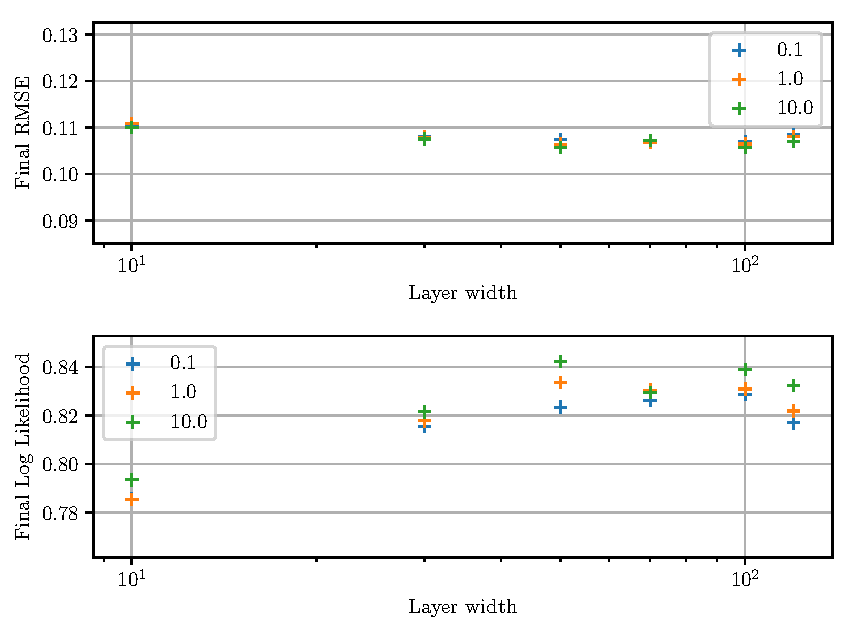
\includegraphics[width=\textwidth]{\dataset/hidden-size}
		\caption{\dataname}
		\label{fig:hidden_width_\dataset}
	\end{subfigure}
	\def\dataset{\concretevar}
	\def\dataname{\concretename}
	\begin{subfigure}{0.48\textwidth}
		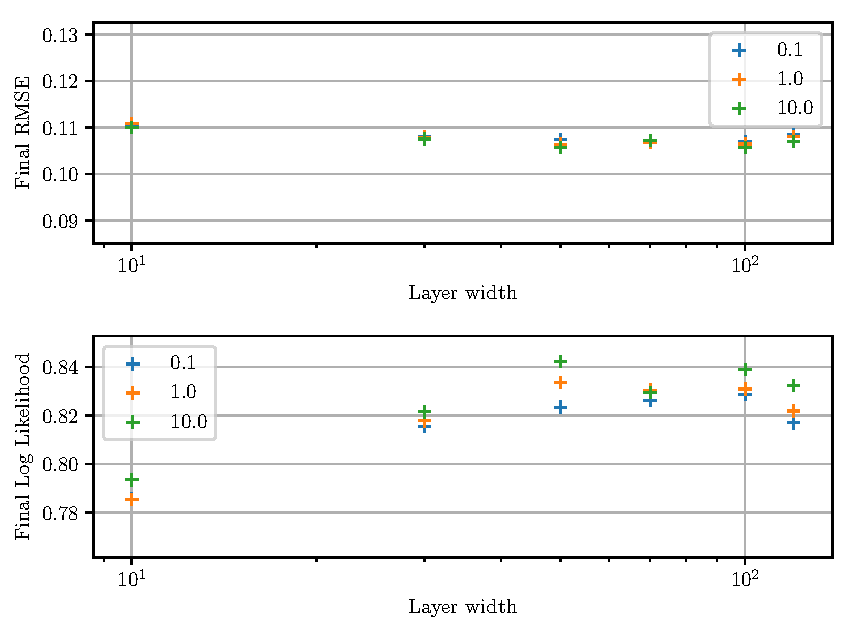
\includegraphics[width=\textwidth]{\dataset/hidden-size}
		\caption{\dataname}
		\label{fig:hidden_width_\dataset}
	\end{subfigure}
	
	\def\dataset{\energyvar}
	\def\dataname{\energyname}
	\begin{subfigure}{0.48\textwidth}
		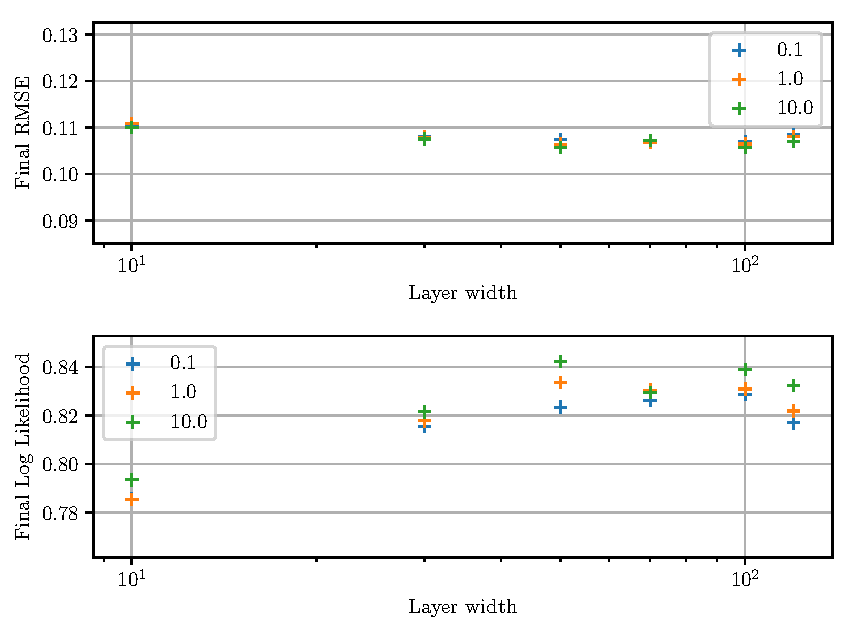
\includegraphics[width=\textwidth]{\dataset/hidden-size}
		\caption{\dataname}
		\label{fig:hidden_width_\dataset}
	\end{subfigure}
	\def\dataset{\kinvar}
	\def\dataname{\kinname}
	\begin{subfigure}{0.48\textwidth}
		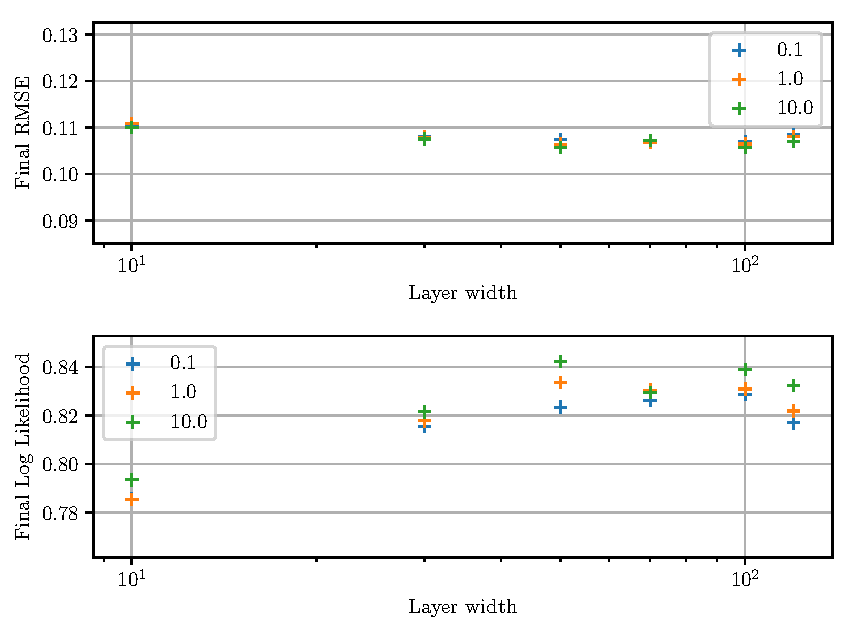
\includegraphics[width=\textwidth]{\dataset/hidden-size}
		\caption{\dataname}
		\label{fig:hidden_width_\dataset}
	\end{subfigure}

	\def\dataset{\powervar}
	\def\dataname{\powername}
	\begin{subfigure}{0.48\textwidth}
		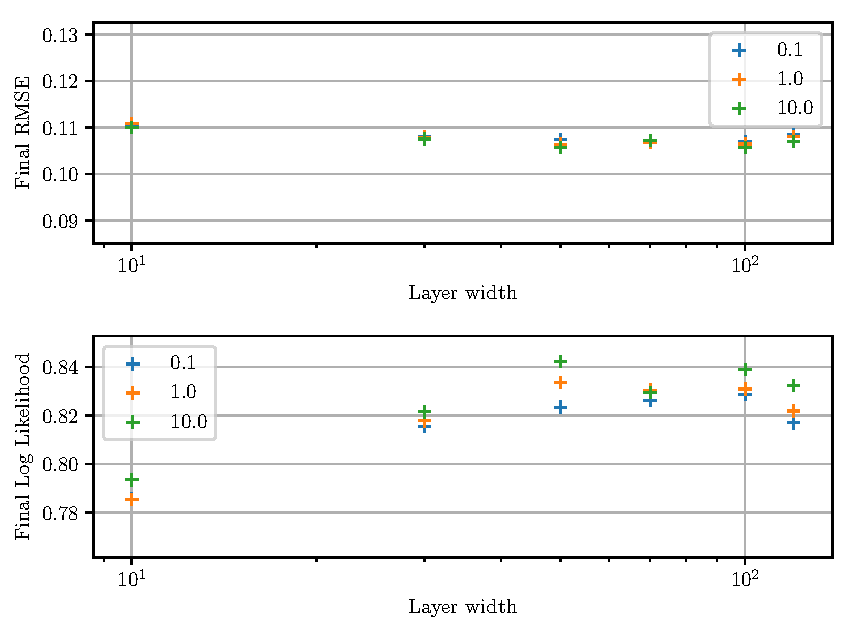
\includegraphics[width=\textwidth]{\dataset/hidden-size}
		\caption{\dataname}
		\label{fig:hidden_width_\dataset}
	\end{subfigure}
	\def\dataset{\proteinvar}
	\def\dataname{\proteinname}
	\begin{subfigure}{0.48\textwidth}
		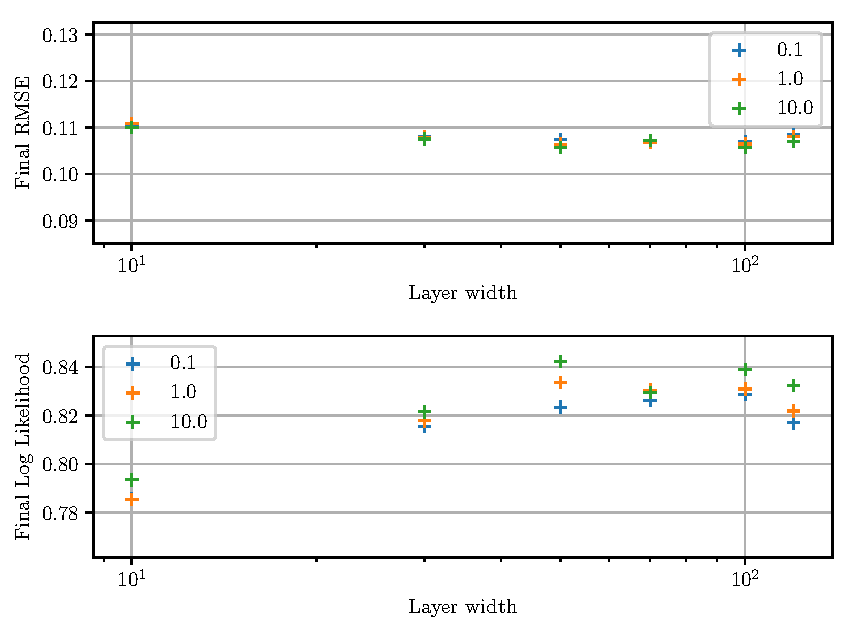
\includegraphics[width=\textwidth]{\dataset/hidden-size}
		\caption{\dataname}
		\label{fig:pruning_\dataset}
	\end{subfigure}
	
	\def\dataset{\winevar}
	\def\dataname{\winename}
	\begin{subfigure}{0.48\textwidth}
		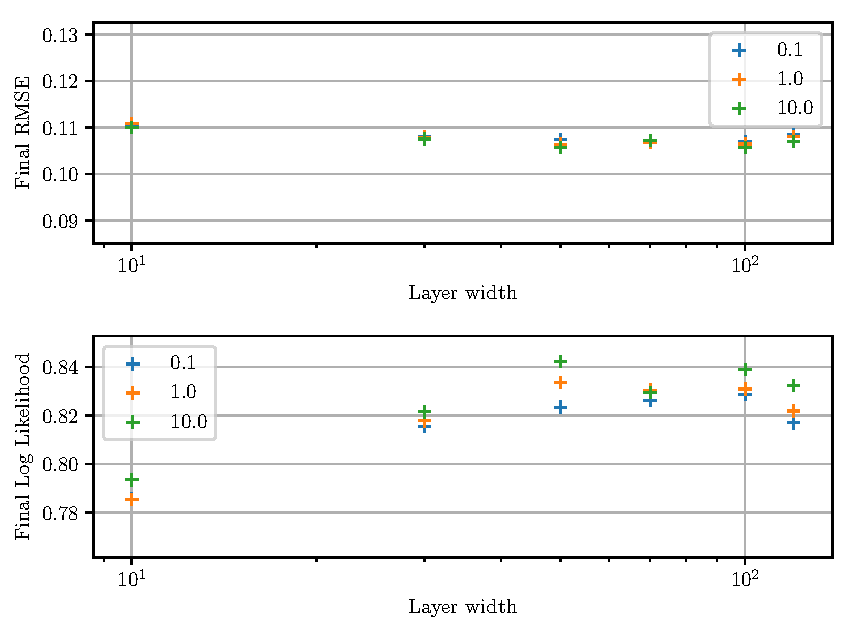
\includegraphics[width=\textwidth]{\dataset/hidden-size}
		\caption{\dataname}
		\label{fig:hidden_width_\dataset}
	\end{subfigure}
	\def\dataset{\yachtnvar}
	\def\dataname{\yachtname}
	\begin{subfigure}{0.48\textwidth}
		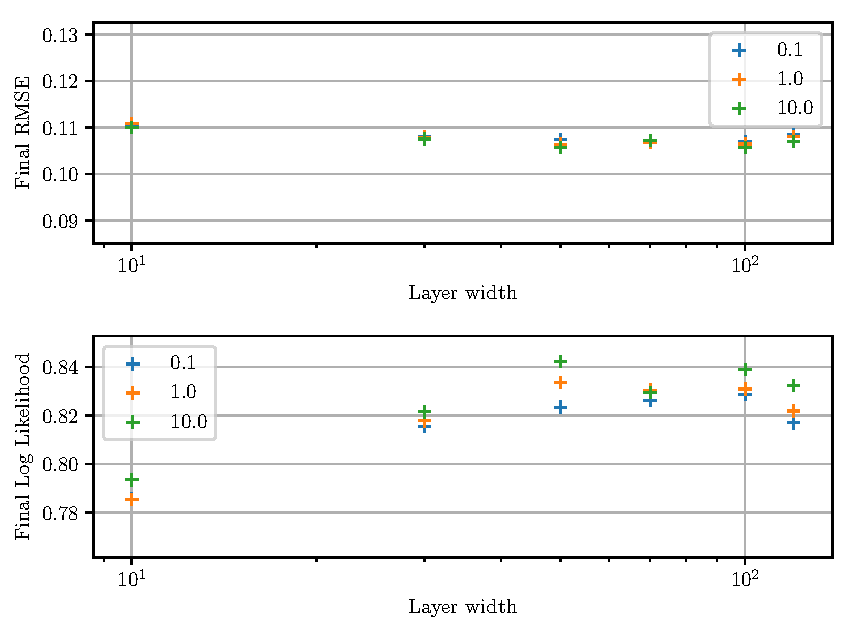
\includegraphics[width=\textwidth]{\dataset/hidden-size}
		\caption{\dataname}
		\label{fig:hidden_width_\dataset}
	\end{subfigure}

	\caption{Final validation log likelihood and RMSE error of various sizes of the hidden layers in 2 layer BNNs. Colour denotes prior width used. Plotted for a number of datasets}
	\label{fig:hidden_width}
\end{figure}

\subsection{Prior width}

Figure \ref{fig:prior_width} details the effects of varying the widths of the prior in 2 layer networks with a fixed architecture. There is again a clear dependency here. For some, the prior width appears to be important up to a particular width, after which it is makes no difference if the width is increased. For some, there is a minor drop off in performance with too large prior width. The clearest trend is that too small a prior width causes significant detriment to performance. This is to be expected. Too small a prior width will over-penalise weights of the size required to produce the required outputs, significantly hampering the model's predictive performance. 

\begin{figure}[p]
	\def\dataset{\bostonvar}
	\def\dataname{\bostonname}
	\begin{subfigure}{0.48\textwidth}
		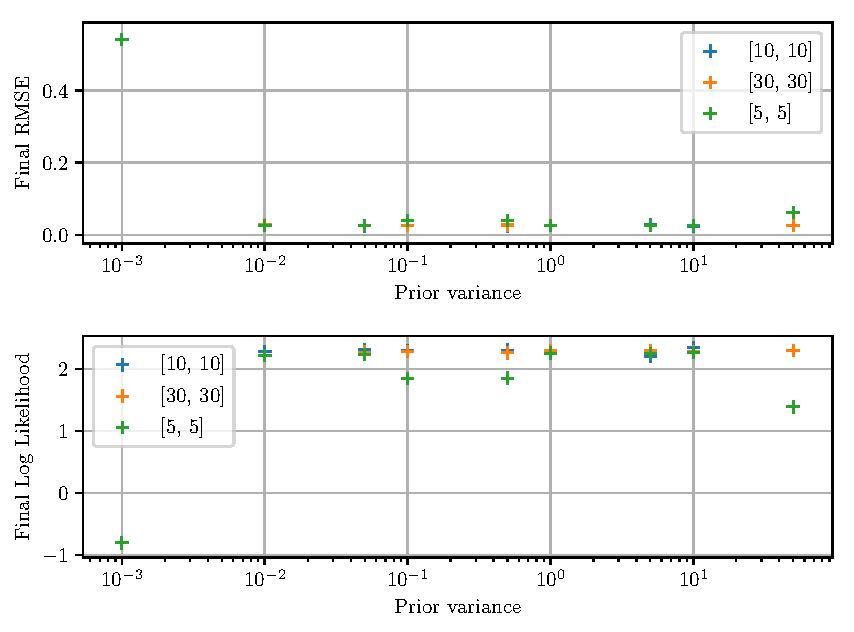
\includegraphics[width=\textwidth]{\dataset/prior-width}
		\caption{\dataname}
		\label{fig:prior_width_\dataset}
	\end{subfigure}
	\def\dataset{\concretevar}
	\def\dataname{\concretename}
	\begin{subfigure}{0.48\textwidth}
		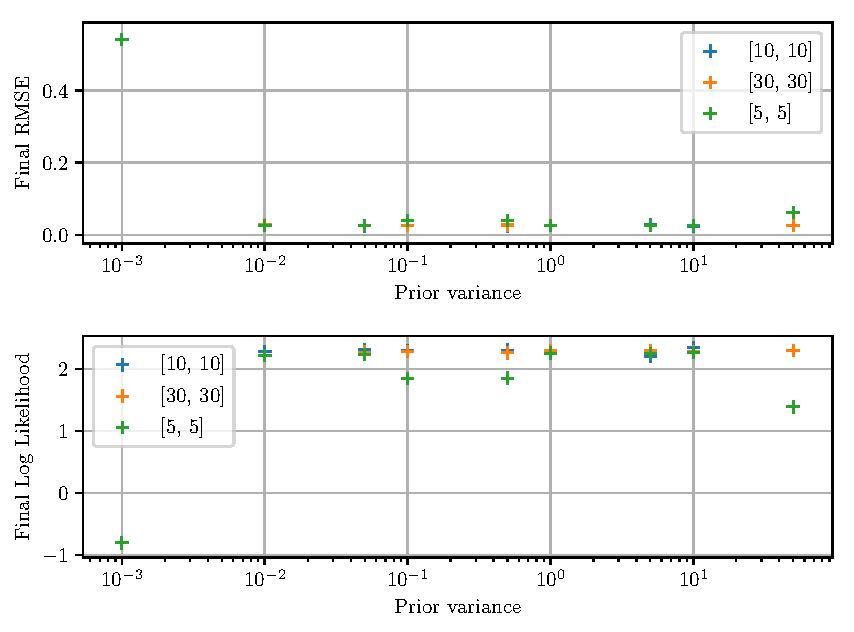
\includegraphics[width=\textwidth]{\dataset/prior-width}
		\caption{\dataname}
		\label{fig:prior_width_\dataset}
	\end{subfigure}

	\def\dataset{\energyvar}
	\def\dataname{\energyname}
	\begin{subfigure}{0.48\textwidth}
		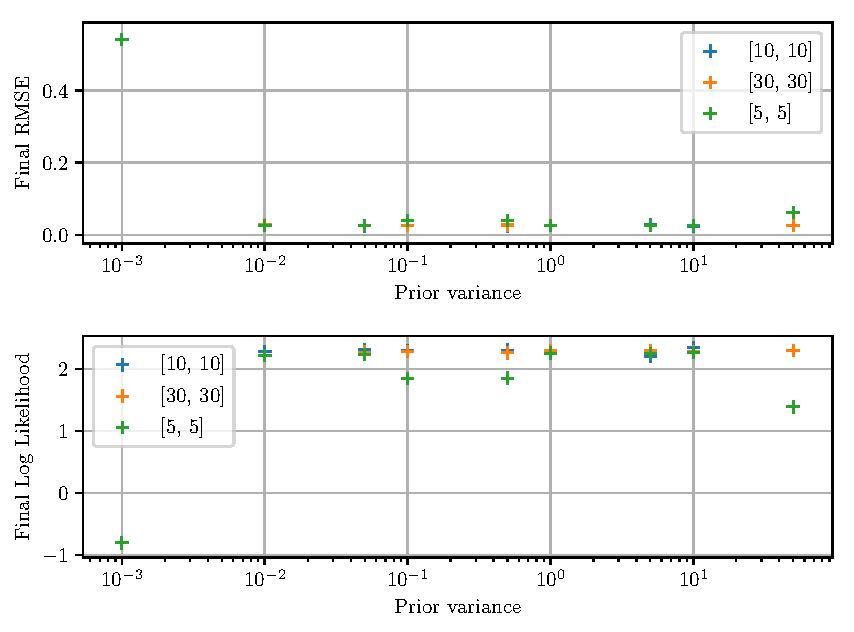
\includegraphics[width=\textwidth]{\dataset/prior-width}
		\caption{\dataname}
		\label{fig:prior_width_\dataset}
	\end{subfigure}
	\def\dataset{\kinvar}
	\def\dataname{\kinname}
	\begin{subfigure}{0.48\textwidth}
		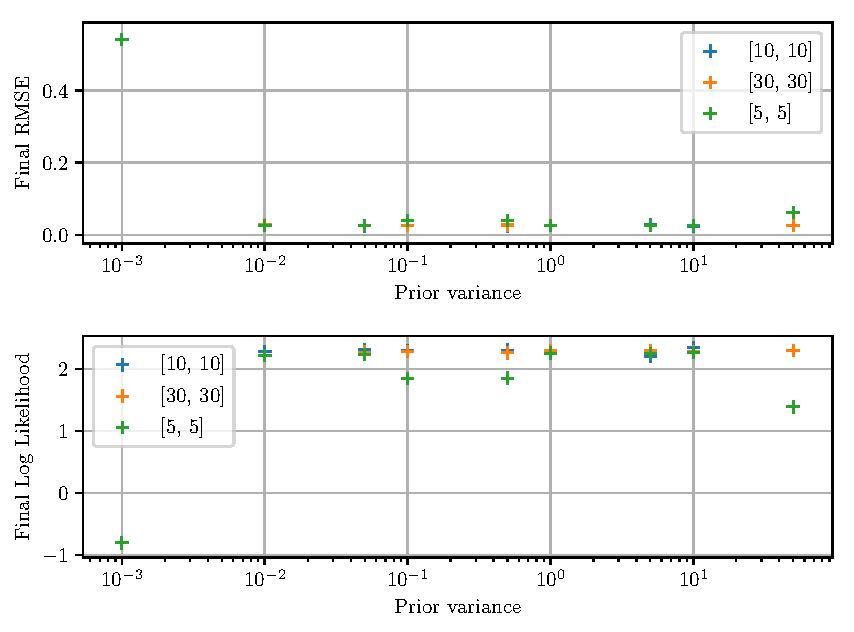
\includegraphics[width=\textwidth]{\dataset/prior-width}
		\caption{\dataname}
		\label{fig:prior_width_\dataset}
	\end{subfigure}
	
	\def\dataset{\powervar}
	\def\dataname{\powername}
	\begin{subfigure}{0.48\textwidth}
		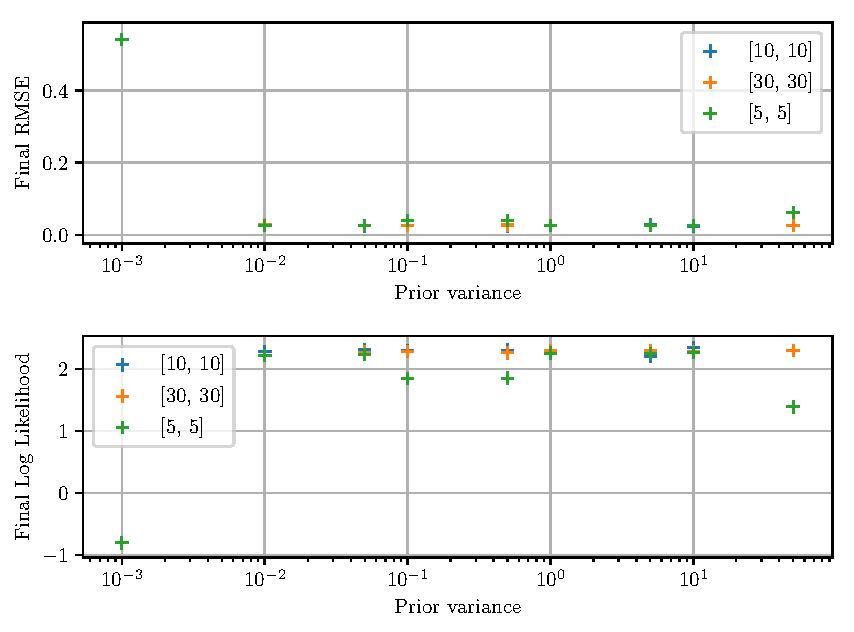
\includegraphics[width=\textwidth]{\dataset/prior-width}
		\caption{\dataname}
		\label{fig:prior_width_\dataset}
	\end{subfigure}
	\def\dataset{\proteinvar}
	\def\dataname{\proteinname}
	\begin{subfigure}{0.48\textwidth}
		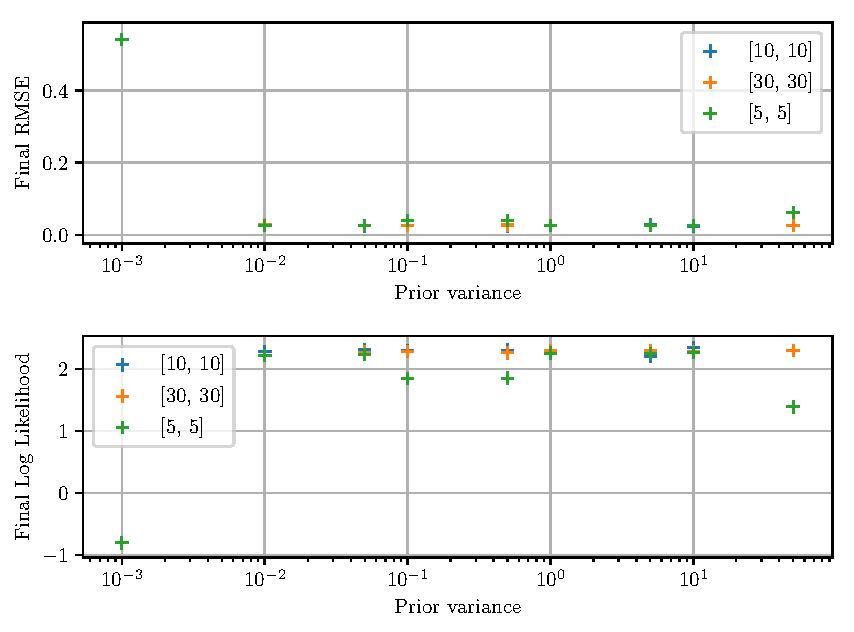
\includegraphics[width=\textwidth]{\dataset/prior-width}
		\caption{\dataname}
		\label{fig:prior_width_\dataset}
	\end{subfigure}
	
	\def\dataset{\winevar}
	\def\dataname{\winename}
	\begin{subfigure}{0.48\textwidth}
		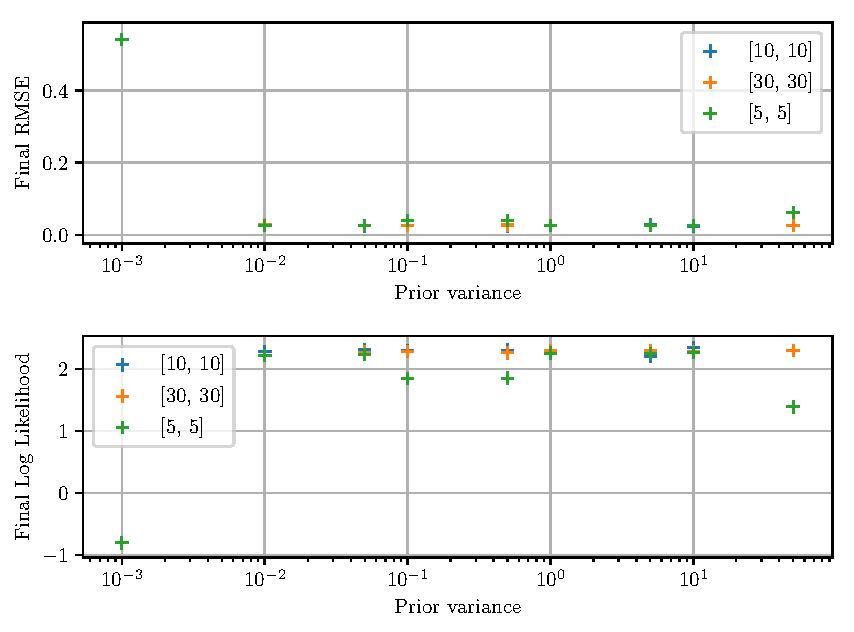
\includegraphics[width=\textwidth]{\dataset/prior-width}
		\caption{\dataname}
		\label{fig:prior_width_\dataset}
	\end{subfigure}
	\def\dataset{\yachtnvar}
	\def\dataname{\yachtname}
	\begin{subfigure}{0.48\textwidth}
		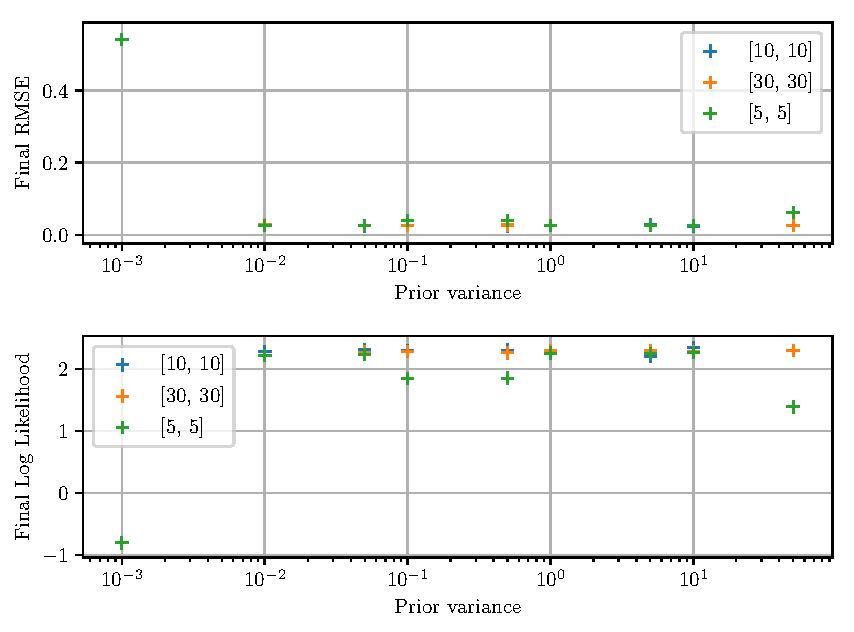
\includegraphics[width=\textwidth]{\dataset/prior-width}
		\caption{\dataname}
		\label{fig:prior_width_\dataset}
	\end{subfigure}
	
	\caption{Final validation log likelihood and RMSE error of various prior widths in 2 layer BNNs. Colour denotes network structure. Plotted for a number of datasets}
	\label{fig:prior_width}
\end{figure}

\subsection{Initialisation of \( \sigma_y^2 \)}

The final parameter investigated in this manner is the initial homoeoskedastic noise on the output of the network, \( y \sim \mathcal{N}(f_\mu(\mathbf{x}), \sigma_y^2) \). Initialisation of this parameter appeared to have little effect on the final performance of the network. There was some effect on the convergence rate of the network. Generally larger \( \sigma_y \) converged faster, but this trend wasn't conclusive. Given the lack of effect on the final performance of the network, it is omitted from the architecture search.

\section{Data Augmentation to control over-fitting and under-fitting}
\label{sec:dataaug}

\begin{figure}[t]
	\begin{subfigure}{0.48\textwidth}
		\def\dataset{\bostonvar}
		\def\dataname{\bostonname}
		\centering
		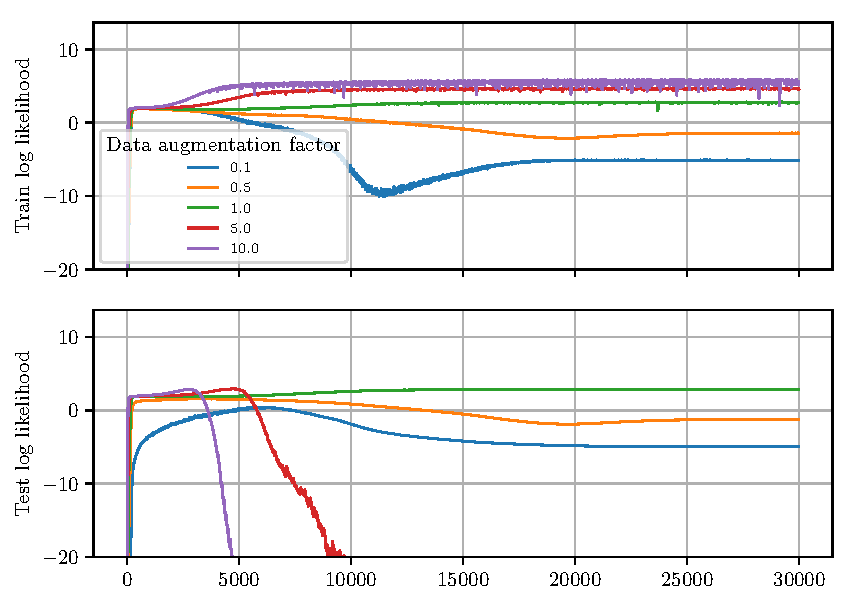
\includegraphics[width=\textwidth]{\dataset/data-multiply-combined}
		\caption{\dataname}
		\label{fig:data_multiply_\dataset}
	\end{subfigure}
%	\begin{subfigure}{0.48\textwidth}
%		\def\dataset{\concretevar}
%		\def\dataname{\concretename}
%		\centering
%		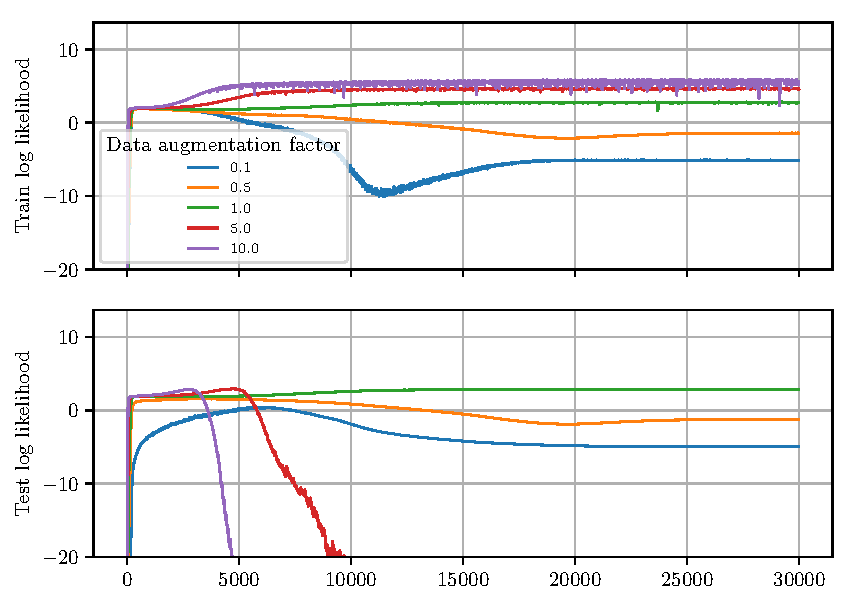
\includegraphics[width=\textwidth]{\dataset/data-multiply-combined}
%		\caption{\dataname}
%		\label{fig:data_multiply_\dataset}
%	\end{subfigure}
%	
	\begin{subfigure}{0.48\textwidth}
		\def\dataset{\energyvar}
		\def\dataname{\energyname}
		\centering
		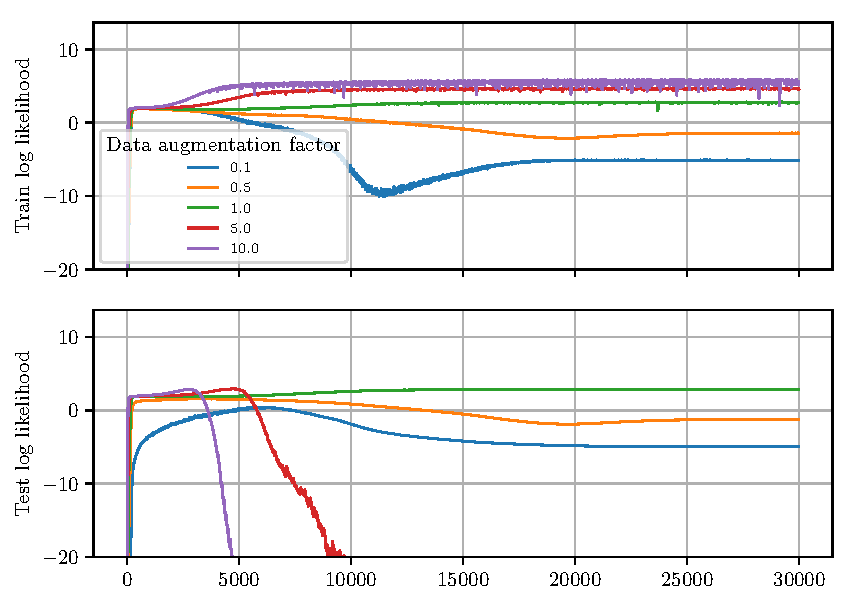
\includegraphics[width=\textwidth]{\dataset/data-multiply-combined}
		\caption{\dataname}
		\label{fig:data_multiply_\dataset}
	\end{subfigure}
%	\begin{subfigure}{0.48\textwidth}
%		\def\dataset{\kinvar}
%		\def\dataname{\kinname}
%		\centering
%		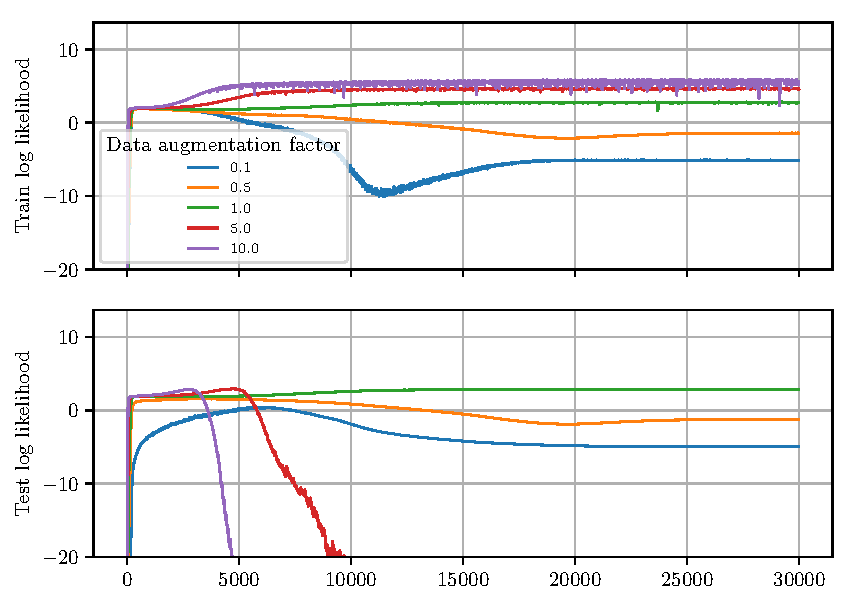
\includegraphics[width=\textwidth]{\dataset/data-multiply-combined}
%		\caption{\dataname}
%		\label{fig:data_multiply_\dataset}
%	\end{subfigure}
%	
%	\begin{subfigure}{0.48\textwidth}
%		\def\dataset{\powervar}
%		\def\dataname{\powername}
%		\centering
%		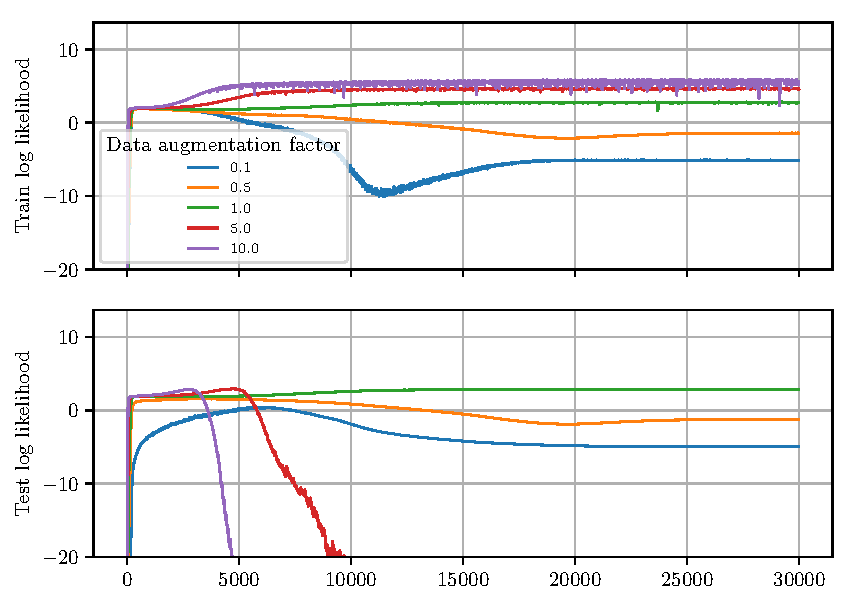
\includegraphics[width=\textwidth]{\dataset/data-multiply-combined}
%		\caption{\dataname}
%		\label{fig:data_multiply_\dataset}
%	\end{subfigure}
%	\begin{subfigure}{0.48\textwidth}
%		\def\dataset{\proteinvar}
%		\def\dataname{\proteinname}
%		\centering
%		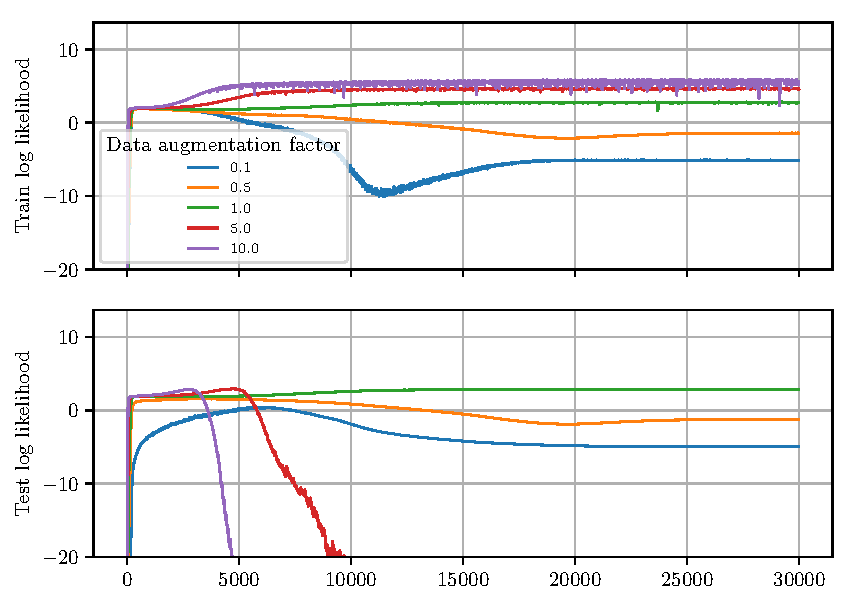
\includegraphics[width=\textwidth]{\dataset/data-multiply-combined}
%		\caption{\dataname}
%		\label{fig:data_multiply_\dataset}
%	\end{subfigure}
%	
	\begin{subfigure}{0.48\textwidth}
		\def\dataset{\winevar}
		\def\dataname{\winename}
		\centering
		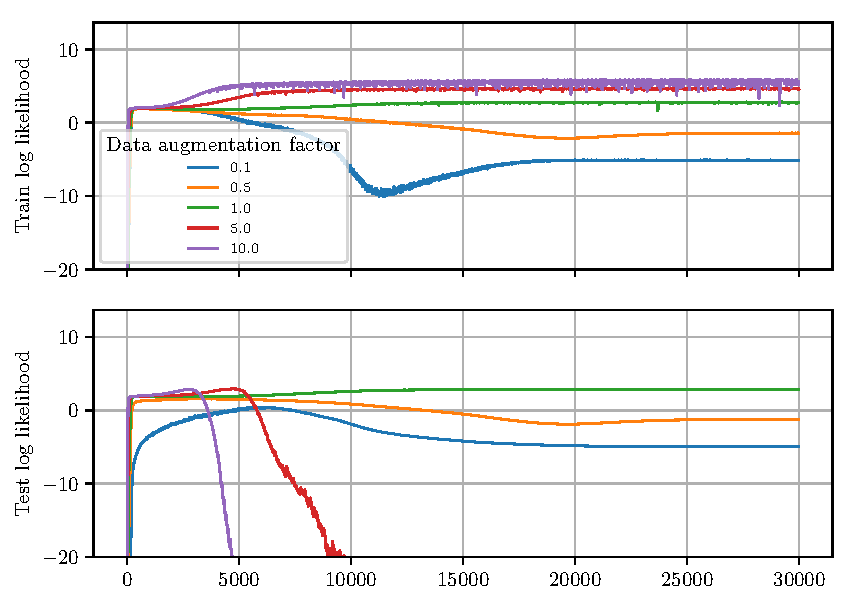
\includegraphics[width=\textwidth]{\dataset/data-multiply-combined}
		\caption{\dataname}
		\label{fig:data_multiply_\dataset}
	\end{subfigure}
	\begin{subfigure}{0.48\textwidth}
		\def\dataset{\yachtnvar}
		\def\dataname{\yachtname}
		\centering
		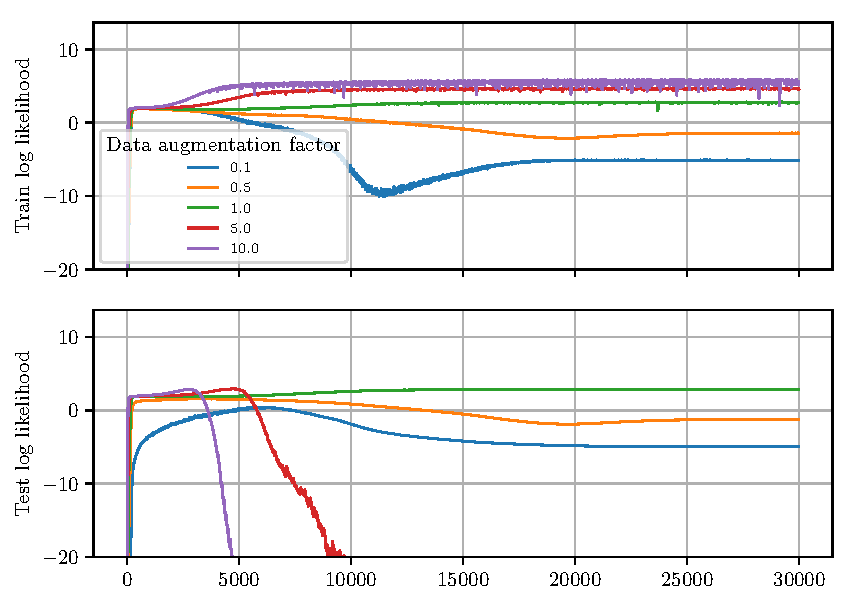
\includegraphics[width=\textwidth]{\dataset/data-multiply-combined}
		\caption{\dataname}
		\label{fig:data_multiply_\dataset}
	\end{subfigure}
	\caption{The effects of modifying the amount of data in a dataset on the train and test log likelihood for a fixed network size. Upper plots show the train set log likelihood through optimisation, and the lower plots the validation log likelihood. With too little,or too much data we see the effects of under-fitting (reduced train and test log likelihood) and over-fitting (increased train log likelihood, significantly decreased test log likelihood) respectively.}
	\label{fig:datamultiply}
\end{figure}

One explanation for the drop-off in performance with larger network size comes from the scaling of the terms in the ELBO cost. The two main terms are the reconstruction loss and the prior fit terms.
\begin{align}
	\ELBO = \underbrace{\E_{q_\phi(\mathbf{w})}\left[ \log P(\mathbf{y} |  \mathbf{w}, \mathbf{x}) \right]}_{\text{reconstruction loss}} - \underbrace{\DKL{q_\phi(\mathbf{w})}{P(\mathbf{w})}}_{\text{prior fit}}
\end{align}
The reconstruction loss is a sum over the log likelihood of the individual data points in the data set, scaling with the quantity of data This term rewards good fit to the data. The prior fit term is a sum over the KL divergence of individual weights (when using a prior with no dependence between weights), therefore scaling with the number of weights in the network. This term rewards keeping the weights close to the prior. 

If we consider a fixed network architecture, we should therefore expect the optimal weights of the network to vary with the amount of data set, as the balance between the two cost terms changes. With a large data-to-network size ratio, we would expect the reconstruction term to overpower the prior fit, resulting in an emphasis on fitting to the train set and potentially over-fitting. With low data-to-network size ratio, we should expect a prioritisation of the prior fit term and a potential for under-fitting. A balance between these terms will give optimal validation set performance. 

In order to test this, the architectures and prior widths that gave optimal performance in the previous experiments were taken. The training datasets were then either under-sampled by some factor by random selection, or over sampled by repeating the dataset and shuffling randomly. The networks were then trained on the new datasets and evaluated on the original validation sets.

Figure \ref{fig:datamultiply} shows the results of these experiments on 4 datasets. We observe the clear signs of under-fitting for low amounts of data - slightly reduced train and validation log likelihood in final performance, and over-fitting with large amounts of data - raised train log likelihood but severely dropped validation log likelihood. We can propose that the under-fitting is likely due to over-regularisation by the KL term and not due to a lack of data by observing that during training, the validation likelihood generally reaches the optimal performance, before being push off from this optima later in training. 

These results help explain the existence of optimal network size being at some finite size, as opposed to an infinite size.

The implications for architecture search are that the size of the network will play a significant role in the performance, in combination with the underlying connective structure. Too large networks will likely systematically under-fit due to over-regularisation by the prior fit term, and small will networks over-fit. 

This does present an interesting method to investigate for restricted size networks, e.g. on embedded devices. Given that for small networks too much data in the training set will cause over-fitting, reducing the amount of data to an empirically appropriate level could see significant performance gains.

\section{Pruning effects in mean-field BNNs}
\label{sec:pruning}

A question raised by the previous section is how the trade-off is being made between the two terms in the ELBO loss, in terms of the weight distributions.

This is investigated by looking at the weights associated with a given hidden unit. Looking at the KL divergence between the weights and the prior, we can investigate how "active" a given weight is. A low KL would indicate that the weight is close to the prior, i.e. close to zero mean and with a width close to the prior, unlikely to be contributing to the performance of the network. A higher KL would indicate the weight is sufficiently dissimilar from the prior. By averaging the KL of all incoming weights to a unit, we can get a measure of the activity of a given neuron. 

The BNNs trained in this experiment utilise the VI training framework with mean field Gaussian priors, utilising Inverse-Gamma hyper-priors on the prior width, with Inverse-Gamma parameters \( \alpha=4.4798, \beta=5.4798 \) (recommended by \citet{wu2018fixing}). They are optimised with the ADAM optimiser, with the settings learning rate=0.001, \( \beta_1 \)=0.9, \( \beta_2 \)=0.999, \( \epsilon \)=1e-8.

Figure \ref{fig:pruning_hist} show example histograms of the distribution of the average KL per neuron. We can clearly see two distinct groups emerge. A larger group, comprising of inactive neurons, and a much smaller group showing the active neurons. Given the very small mean KLs of the weights in the larger group, they are unlikely to contribute significantly to the predictions of the network. We can therefore consider these neurons inactive, or pruned. By placing an appropriate threshold on the value of the average KL for a neuron, we can count the number of total active neurons in a network. 

\begin{figure}
	\centering
	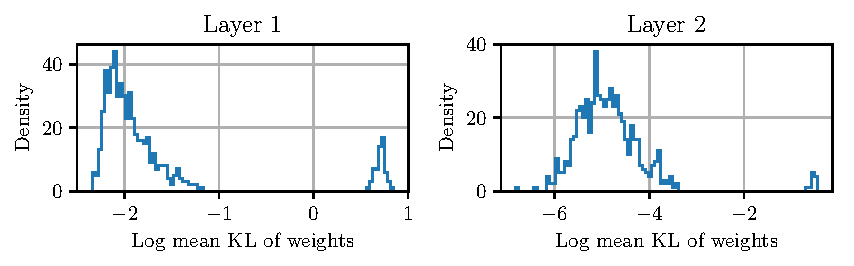
\includegraphics{pruning_example}
	\caption{Histogram of the log mean KL of the weights associated with a give neuron in a 2 layer, 600 unit per layer network trained on the \proteinname \: dataset. Each histogram is for the units of a give layer. Clearly visible is the splitting of the units into two groups, the active and the inactive.}
	\label{fig:pruning_hist}
\end{figure}

Figures \ref{fig:pruning_1} and \ref{fig:pruning_2} detail the results of training various networks on 8 UCI datasets. Networks are defined by a number of layers, and the same hidden width for every layer. Networks of various widths and depths are tested, as appropriate to the specific dataset.

Clearly visible we can see trends in the pruning effect. The number of active neurons increases with network size, utilising all neurons available, up to a point. Past a given break point there is a decreases in the number of neurons effectively utilised. There is a sharp discontinuity in many of these plots in the number of neurons utilised. This comes from the difficulty in exactly defining the boundary of what the threshold is for a neuron to be active. Before this point all neurons are active and so form a single group in the spread of neuron KLs. After this point, two groups exist: the active and inactive. In the transition region between the two, the spread of KL values widens until it separates into the two groups. Defining exactly when to consider neurons inactive is slightly arbitrary, and always leads to the sort of discontinuity seen. 

It is interesting to note that even as fewer neurons become active, in many cases the validation performance of the network continues to increase slightly. This is likely due to the extra regularisation provided by the removal of additional neurons causing the network to generalise better than networks that are slightly smaller. In the limit of large networks, one of two effects appears to present. Either the performance of the network flat-lines, or we see a decrease in performance. The flat-lining behaviour is what we would hope to see in a Bayesian method. For smaller models, adding more units increases the model's capacity to explain the data. Once sufficient capacity is reached, the Bayesian method prunes out the unwanted extra capacity. 

The decrease in performance seen on some datasets is not explained by this interpretation. One theory to explain this is the additional Monte Carlo noise that the pruned units enter into the gradient estimates. While pruned weights have zero mean, they still have a variance and so will likely have some magnitude when sampled. More pruned units will cause more noise. If the optimisation is difficult (i.e. it is a difficult function to learn) it may become increasingly difficult for the optimiser to make headway towards an optimal model in light of noisy gradients, reducing performance. Investigating optimisers other than ADAM may provide more answers.
	
Another point of interest is that these trends tend to match with the width of the network, rather than with the total number of neurons or weights in the network. Further investigation into the pruning in individual layers of the network shows that most active neurons are in the first layer of the network, with significantly fewer in later layers. This would imply that the size of the first layer of the network is the bottle-neck in performance in this case, and that subsequent layers need not be as wide, as per conventional methodology. This is a potential deficiency of the search space  used, with all layers the same size proposed for this project. An alternative to this that attempts to resolve this issue does not change the methodology is proposed earlier.

\begin{figure}[ph]
	\def\dataset{\bostonvar}
	\def\dataname{\bostonname}
	\begin{subfigure}{0.48\textwidth}
		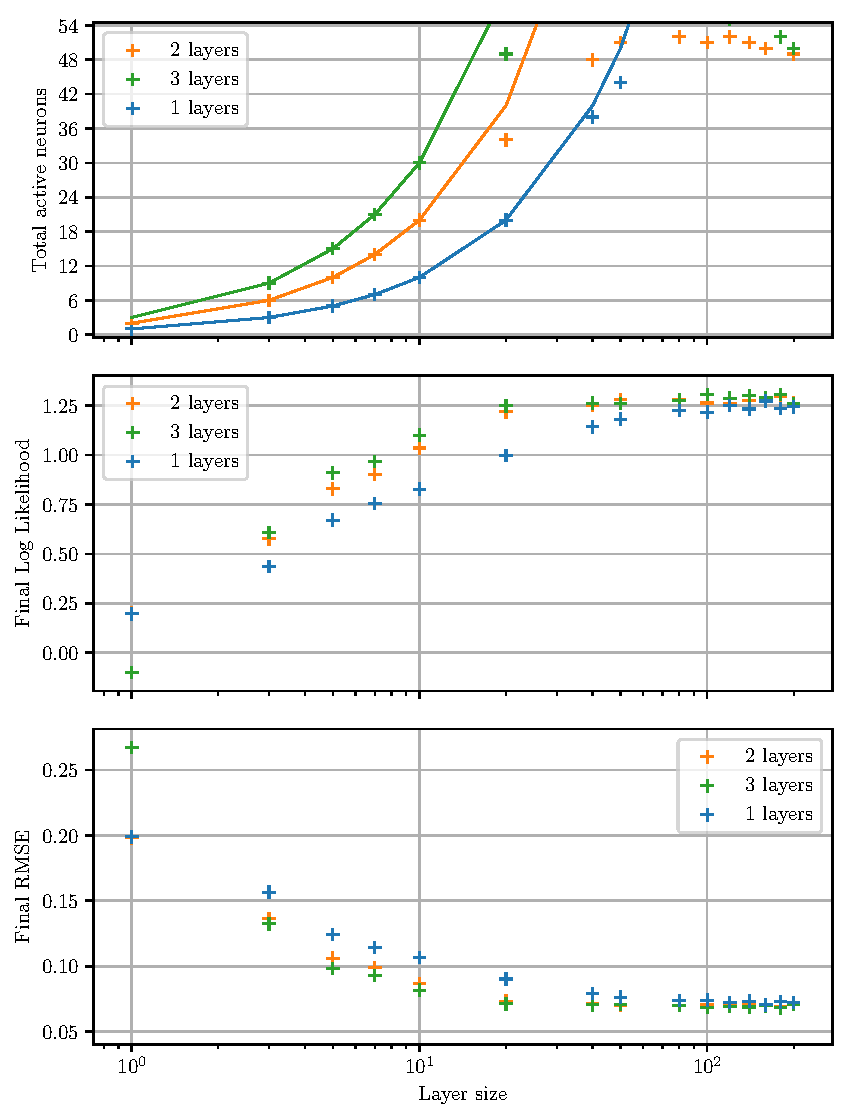
\includegraphics[width=\textwidth]{\dataset/pruning_combined}
		\caption{\dataname}
		\label{fig:pruning_\dataset}
	\end{subfigure}
	\def\dataset{\concretevar}
	\def\dataname{\concretename}
	\begin{subfigure}{0.48\textwidth}
		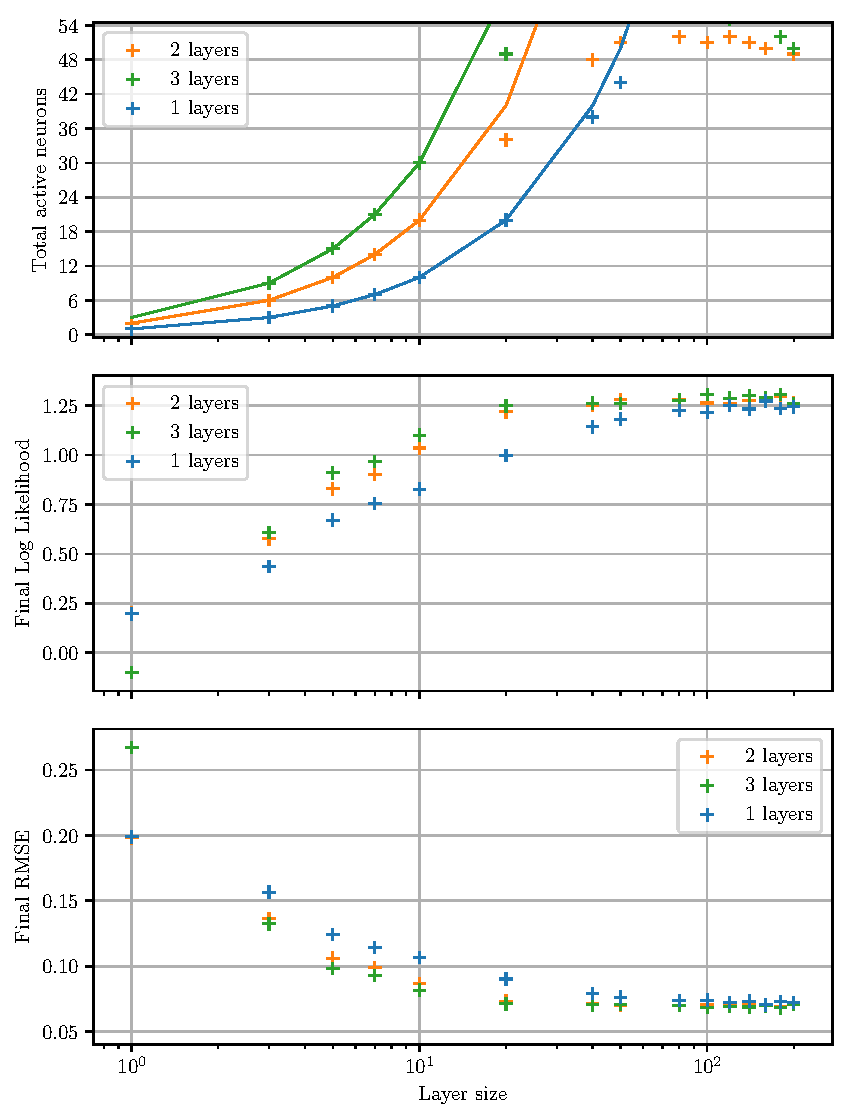
\includegraphics[width=\textwidth]{\dataset/pruning_combined}
		\caption{\dataname}
		\label{fig:pruning_\dataset}
	\end{subfigure}
	
	\def\dataset{\energyvar}
	\def\dataname{\energyname}
	\begin{subfigure}{0.48\textwidth}
		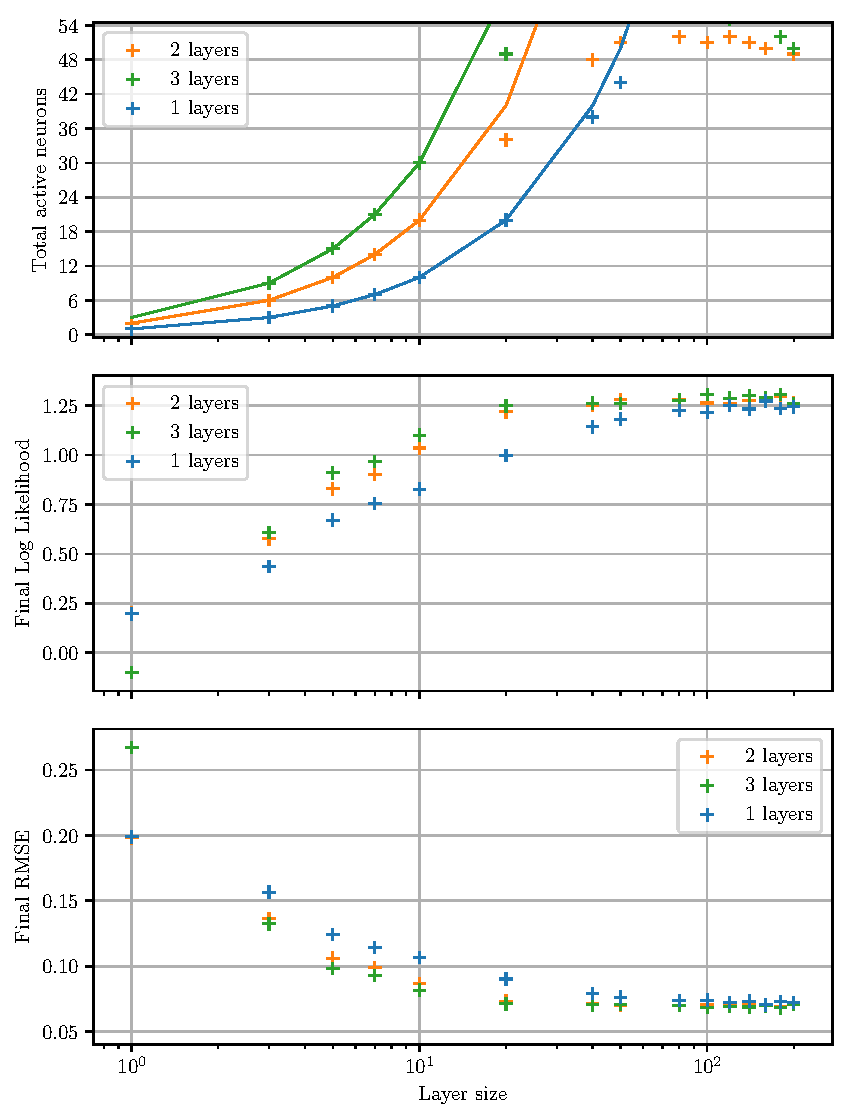
\includegraphics[width=\textwidth]{\dataset/pruning_combined}
		\caption{\dataname}
		\label{fig:pruning_\dataset}
	\end{subfigure}
	\def\dataset{\kinvar}
	\def\dataname{\kinname}
	\begin{subfigure}{0.48\textwidth}
		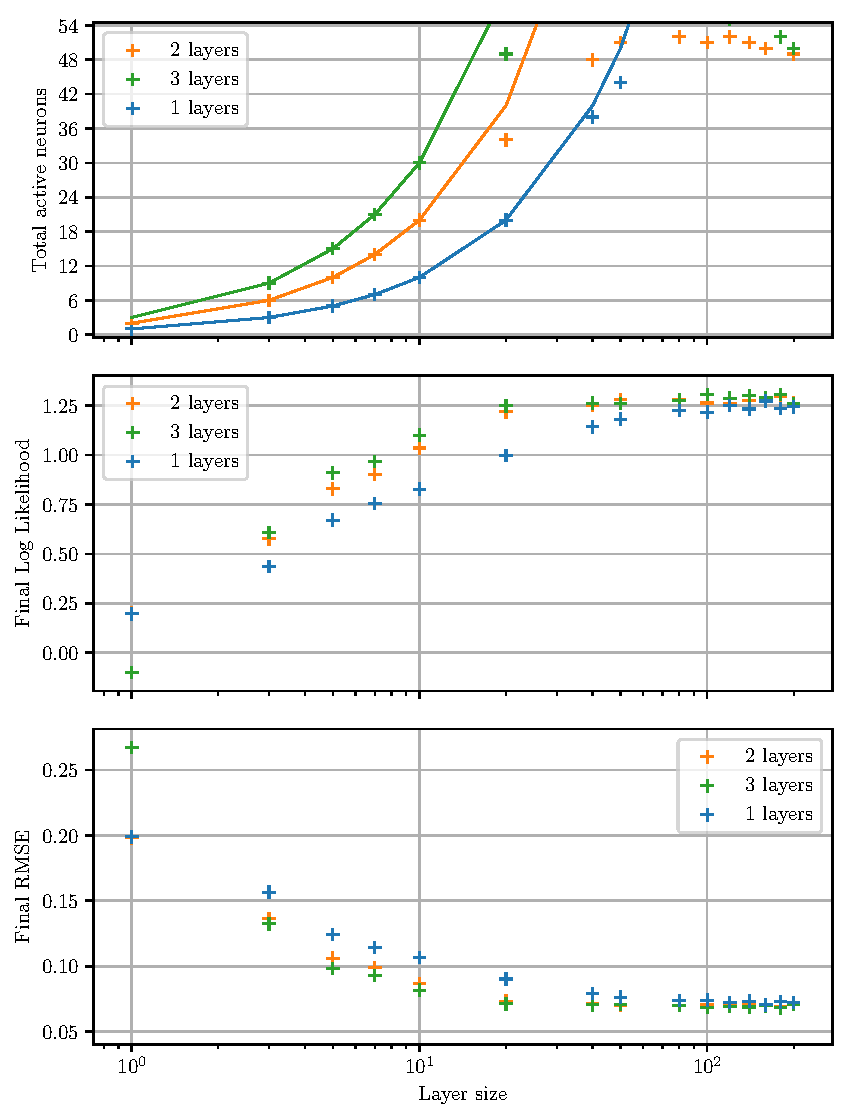
\includegraphics[width=\textwidth]{\dataset/pruning_combined}
		\caption{\dataname}
		\label{fig:pruning_\dataset}
	\end{subfigure}
	\caption{Plots detailing the effect of pruning in VI BNNs on various datasets for a range of architectures. Upper plots show the number of units active in the network, defined by the average KL of units input weights. Solid lines show the total number of units available in the network. Middle plots show the average log likelihood over the last 20 optimisation steps of the network. Lower plots show the average RMSE error over the last 20 optimisation steps of the network. Here we see clearly the effects of model pruning occurring, with the number of active unit in a given model remaining limited with increasing model size. A corresponding effect on performance is seen.}
	\label{fig:pruning_1}
\end{figure}

\begin{figure}[ph]
	\def\dataset{\powervar}
	\def\dataname{\powername}
	\begin{subfigure}{0.48\textwidth}
		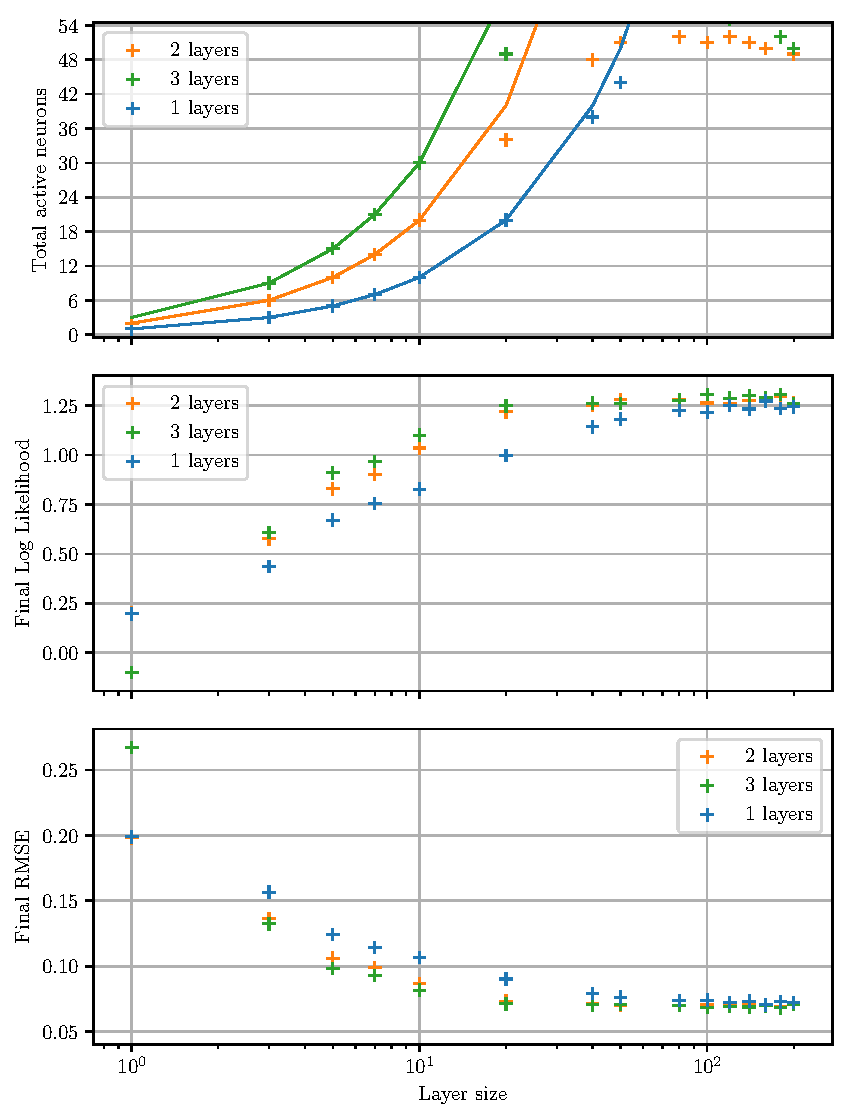
\includegraphics[width=\textwidth]{\dataset/pruning_combined}
		\caption{\dataname}
		\label{fig:pruning_\dataset}
	\end{subfigure}
	\def\dataset{\proteinvar}
	\def\dataname{\proteinname}
	\begin{subfigure}{0.48\textwidth}
		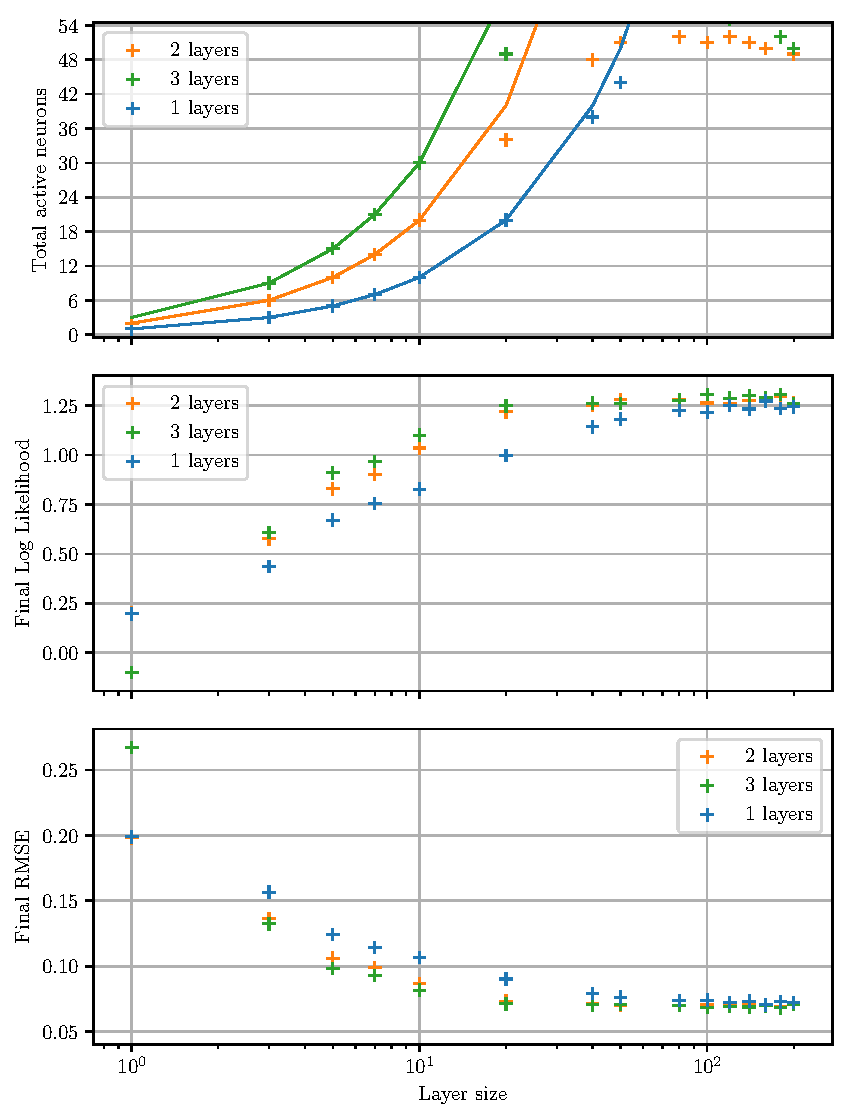
\includegraphics[width=\textwidth]{\dataset/pruning_combined}
		\caption{\dataname}
		\label{fig:pruning_\dataset}
	\end{subfigure}
	
	\def\dataset{\winevar}
	\def\dataname{\winename}
	\begin{subfigure}{0.48\textwidth}
		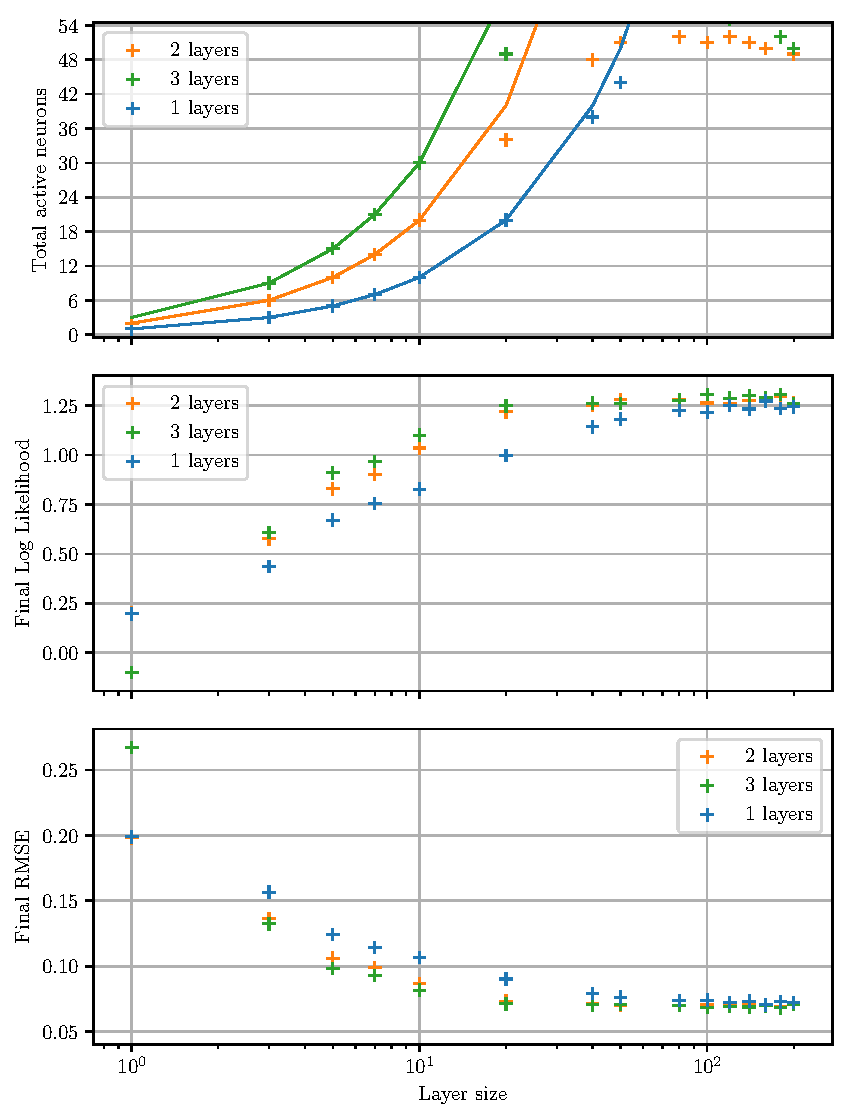
\includegraphics[width=\textwidth]{\dataset/pruning_combined}
		\caption{\dataname}
		\label{fig:pruning_\dataset}
	\end{subfigure}
	\def\dataset{\yachtnvar}
	\def\dataname{\yachtname}
	\begin{subfigure}{0.48\textwidth}
		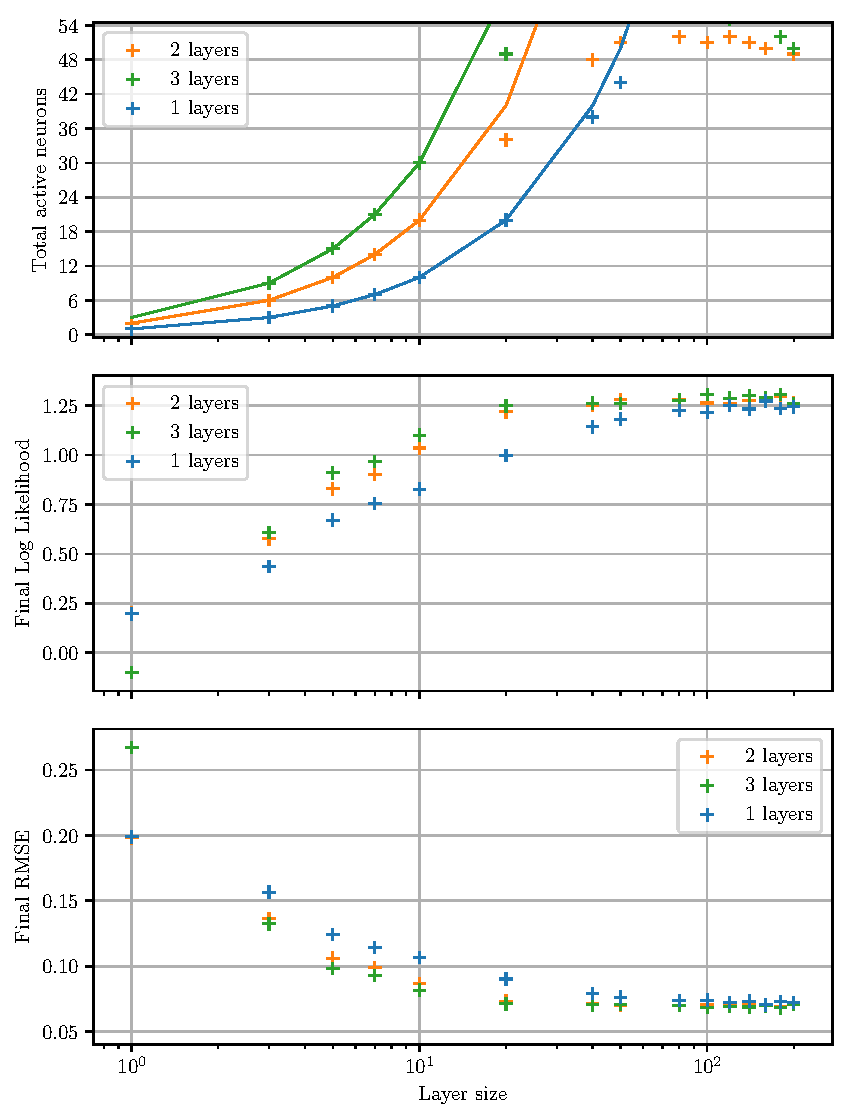
\includegraphics[width=\textwidth]{\dataset/pruning_combined}
		\caption{\dataname}
		\label{fig:pruning_\dataset}
	\end{subfigure}
	\caption{Plots detailing the effect of pruning in VI BNNs on various datasets for a range of architectures. Upper plots show the number of units active in the network, defined by the average KL of units input weights. Solid lines show the total number of units available in the network. Middle plots show the average log likelihood over the last 20 optimisation steps of the network. Lower plots show the average RMSE error over the last 20 optimisation steps of the network. Here we see clearly the effects of model pruning occurring, with the number of active unit in a given model remaining limited with increasing model size. A corresponding effect on performance is seen.}
	\label{fig:pruning_2}
\end{figure}

\section{Empirical kernel and hyper-parameter selection for GPAR models of architecture performance}
\label{sec:model}

Gaussian Process model fitting is a non-trivial task. To do some one must pick appropriate kernels and training hyper-parameters. In the GPAR model there are a number of other considerations, discussed earlier. This section looks to empirically investigate the choice of kernel and hyper-parameters for application to the search space of architecture search. In order to produce a good surrogate model to use in Bayesian Optimisation, it is necessary to find good training setting and kernel choices.

The datasets fitted to are the results of the models trained in the previous section. Three checkpoints are used from the training of the models: 1000 steps, 4000 steps and the final step (typically 30,000-50,000). These points are chosen for two reasons. First from observation the first two points lie in the region where it is not immediately obvious which network will end up with the better performance. Beyond this point models tend to only slowly asymptote to their optima. This makes the modelling task more interesting. Second, it means that the computation saved from early stopping is significant. We only incur the significant additional cost of going from the second output to the final if we believe to to be a good idea in light of the observed training so far. This subset of models define a search space with a discrete set of network deaths and widths over a given range. Each model reported in this section is run on 5 differently selected subsets of data and trained with a different random seed. The results are reported as the mean and standard deviation of results obtained. 

These tests are performed in two sections: investigation into appropriate kernels, and an investigation into the other training settings of the model. It was ensured that the parameters not tested in each experiment were sufficiently good. However, they may not be optimal and so this pair of experiment implicitly assumes that the results of each are reasonably independent of the other settings.

The models are optimised with the L-BFGS-B algorithm, using the implementation from the Python package SciPy.

\subsection{Kernel investigation}

First we investigate the appropriate form of kernel to use. A non-linear EQ kernel is always placed on the input. In addition a combination of some, all, or none of the following are also used, added together: a liner kernel on the inputs \( \mathbf{x} \), a linear kernel on the outputs \( \mathbf{y}_{1:i} \) and a non-linear kernel on the outputs.

Table \ref{tbl:kernel_half} shows the results of fitting these models to a training set of half the dataset, randomly selected. Table \ref{tbl:kernel_small} shows the results of fitting these models to a training set consisting of 10 points from the dataset, randomly selected. Both are then validated on the remaining data and the log likelihood reported. The second table, the low data case, is of particular interest for the architecture search case as we are looking to make good prediction about model performance from just a few samples.

The results of this investigation are inconclusive. When using a large amount of data, there seems to be a preference for using all the possible kernel option, but this still not close to unanimous. In the low data case, the differences in mean are often overshadowed by the standard deviation of the results. The kernel chosen for use in experiments is therefore a non-linear kernel on the inputs and a linear kernel on the outputs as it appears to overall be the best fitting, but this is not completely clear.

\afterpage{%
	\clearpage% Flush earlier floats (otherwise order might not be correct)
	\thispagestyle{empty}% empty page style (?)
	\begin{landscape}
		%\begin{tabular}{lll|rrrrrrr}
		%	\toprule
		%	\multicolumn{3}{c}{Model settings} & \multicolumn{7}{c}{Dataset} \\
		%	Markov length & Input scales tied & Joint trained & bostonHousing & concrete & energy & kin8nm & power-plant & wine-quality-red &   yacht \\
		
		%\begin{tabular}{lll|rrrrrrr}
		%	\toprule
		%	\multicolumn{3}{c}{Kernal settings} & \multicolumn{7}{c}{Dataset} \\\\
		%	\shortstack[l]{Linear kernal\\on inputs} & \shortstack[l]{Linear kernal\\on outputs} & \shortstack[l]{Non-linear kernal\\on outputs} & bostonHousing & concrete & energy & kin8nm & power-plant & wine-quality-red &   yacht \\
		\begin{table}
			\scriptsize
			\begin{tabular}{lll|rrrrrrr}
				\toprule
				\multicolumn{3}{c}{Kernal settings} & \multicolumn{7}{c}{Dataset} \\\\
				\shortstack[l]{Linear kernal\\on inputs} & \shortstack[l]{Linear kernal\\on outputs} & \shortstack[l]{Non-linear kernal\\on outputs} & bostonHousing & concrete & energy & kin8nm & power-plant & wine-quality-red &   yacht \\
				\midrule
				\multirow{4}{*}{False} & \multirow{2}{*}{False} & False &            -2.64 ± 0.351 &  -1.86 ± 0.429 &    -0.649 ± 0.2 &  1.37 ± 0.304 &  -0.437 ± 0.299 &   -0.874 ± 0.246 &    -51 ± 98.7 \\
				&       & True  &            -2.42 ± 0.269 &  -1.75 ± 0.374 &   -0.49 ± 0.211 &  2.87 ± 0.409 &   0.167 ± 0.235 &   -0.554 ± 0.168 &  -48.9 ± 97.7 \\
				\cline{2-10}
				& \multirow{2}{*}{True} & False &            -2.79 ± 0.248 &  -1.82 ± 0.457 &  -0.529 ± 0.222 &    2.97 ± 0.4 &  0.0153 ± 0.245 &   -0.611 ± 0.169 &  -49.1 ± 96.8 \\
				&       & True  &              -2.56 ± 0.3 &  -1.75 ± 0.354 &  -0.391 ± 0.207 &  \textbf{3.12 ± 0.432} &   0.196 ± 0.212 &    -0.57 ± 0.187 &  -52.7 ± 7.68 \\
				\cline{1-10}
				\cline{2-10}
				\multirow{4}{*}{True} & \multirow{2}{*}{False} & False &            -2.64 ± 0.352 &  -1.86 ± 0.429 &  -0.644 ± 0.203 &    1.4 ± 0.31 &  -0.388 ± 0.306 &   -0.797 ± 0.213 &  -50.5 ± 98.3 \\
				&       & True  &            \textbf{-2.41 ± 0.265} &   \textbf{-1.74 ± 0.37} &  -0.489 ± 0.212 &  2.88 ± 0.412 &    0.197 ± 0.26 &    -0.529 ± 0.16 &  -48.7 ± 97.2 \\
				\cline{2-10}
				& \multirow{2}{*}{True} & False &            -2.78 ± 0.303 &  -1.82 ± 0.458 &  -0.527 ± 0.222 &  2.95 ± 0.431 &     0.14 ± 0.13 &     -0.6 ± 0.174 &  -48.7 ± 96.8 \\
				&       & True  &            -2.56 ± 0.284 &   -1.77 ± 0.39 &  \textbf{-0.387 ± 0.208} &    3.1 ± 0.44 &   \textbf{0.245 ± 0.223} &   \textbf{-0.531 ± 0.161} &  \textbf{-48.1 ± 96.9} \\
				\bottomrule
			\end{tabular}
			\caption{The per data-point validation log likelihood of fitting various combinations of kernels to the performance characteristics of BNNs trained on various datasets. Training sets are 50\% of samples randomly selected. Validation set is the remaining data. Each experiment run 5 times with different seeds. The mean and standard deviation of the results are reported.}
			\label{tbl:kernel_half}
		\end{table}
		
		\begin{table}
			\scriptsize
			\begin{tabular}{lll|rrrrrrr}
				\toprule
				\multicolumn{3}{c}{Kernal settings} & \multicolumn{7}{c}{Dataset} \\
				\shortstack[l]{Linear kernal\\on inputs} & \shortstack[l]{Linear kernal\\on outputs} & \shortstack[l]{Non-linear kernal\\on outputs} & bostonHousing & concrete & energy & kin8nm & power-plant & wine-quality-red &   yacht \\
				\midrule
				\multirow{4}{*}{False} & \multirow{2}{*}{False} & False &               -123 ± 242 &  -23.1 ± 25.9 &   -185 ± 386 &  1.49 ± 2.43 &  0.233 ± 2.48 &     -19.9 ± 27.4 &  -3.93E+03 ± 6.83E+03 \\
				&       & True  &               -124 ± 255 &  -22.9 ± 27.3 &  \textbf{-96.6 ± 136} &  3.19 ± 1.25 &   1.27 ± 1.48 &     -19.9 ± 27.8 &  -3.25E+03 ± 5.05E+03 \\
				\cline{2-10}
				& \multirow{2}{*}{True} & False &               -118 ± 234 &  \textbf{-21.2 ± 23.6} &   -580 ± 586 &   2.8 ± 1.37 &   1.37 ± 2.23 &     -33.7 ± 37.9 &  -4.02E+03 ± 6.92E+03 \\
				&       & True  &               -120 ± 241 &  -36.2 ± 32.9 &   -457 ± 451 &  1.11 ± 4.54 &   \textbf{1.71 ± 1.75} &     -33.5 ± 37.9 &  -4.24E+03 ± 7.37E+03 \\
				\cline{1-10}
				\cline{2-10}
				\multirow{4}{*}{True} & \multirow{2}{*}{False} & False &               -123 ± 241 &      -23 ± 26 &   -169 ± 350 &   1.1 ± 2.12 &   0.53 ± 1.96 &     -19.8 ± 27.4 &   -3.92E+03 ± 6.8E+03 \\
				&       & True  &               \textbf{-105 ± 210} &    -24 ± 29.3 &   -144 ± 207 &  2.78 ± 1.47 &    1.31 ± 1.5 &     -19.7 ± 27.9 &  \textbf{-3.18E+03 ± 5.09E+03} \\
				\cline{2-10}
				& \multirow{2}{*}{True} & False &               -121 ± 242 &  -21.3 ± 24.4 &   -379 ± 531 &  2.97 ± 1.35 &   1.34 ± 2.21 &     -19.8 ± 27.4 &     -4E+03 ± 6.88E+03 \\
				&       & True  &               -120 ± 243 &  -24.6 ± 24.6 &   -210 ± 296 &  \textbf{3.22 ± 1.14} &   1.63 ± 1.57 &     \textbf{-19.6 ± 27.8} &  -4.14E+03 ± 7.16E+03 \\
				\bottomrule
			\end{tabular}
			\caption{The per data-point validation log likelihood of fitting various combinations of kernels to the performance characteristics of BNNs trained on various datasets. Training sets are 10 samples randomly selected. Validation set is the remaining data. Each experiment run 5 times with different seeds. The mean and standard deviation of the results are reported.}
			\label{tbl:kernel_small}
		\end{table}
		
		\clearpage
		
		\begin{table}
			\scriptsize
			\begin{tabular}{lll|rrrrrrr}
				\toprule
				\multicolumn{3}{c}{Model settings} & \multicolumn{7}{c}{Dataset} \\
				Markov length & Input scales tied & Joint trained & bostonHousing & concrete & energy & kin8nm & power-plant & wine-quality-red &   yacht \\
				\midrule
				\multirow{4}{*}{False} & \multirow{2}{*}{False} & False &            -2.64 ± 0.351 &  -1.86 ± 0.429 &    -0.649 ± 0.2 &  1.37 ± 0.304 &  -0.437 ± 0.299 &   -0.874 ± 0.246 &    -51 ± 98.7 \\
				&       & True  &            \textbf{-2.42 ± 0.269} &  \textbf{-1.75 ± 0.374} &   -0.49 ± 0.211 &  2.87 ± 0.409 &   0.167 ± 0.235 &   -0.554 ± 0.168 &  -48.9 ± 97.7 \\
				\cline{2-10}
				& \multirow{2}{*}{True} & False &            -2.79 ± 0.248 &  -1.82 ± 0.457 &  -0.529 ± 0.222 &    2.97 ± 0.4 &  0.0153 ± 0.245 &   -0.611 ± 0.169 &  -49.1 ± 96.8 \\
				&       & True  &              -2.56 ± 0.3 &  \textbf{-1.75 ± 0.354} &  \textbf{-0.391 ± 0.207} &  \textbf{3.12 ± 0.432} &   0.196 ± 0.212 &    -0.57 ± 0.187 &  -5.27 ± 7.68 \\
				\cline{1-10}
				\cline{2-10}
				\multirow{4}{*}{True} & \multirow{2}{*}{False} & False &            -2.64 ± 0.352 &  -1.86 ± 0.429 &  -0.644 ± 0.203 &    1.4 ± 0.31 &  -0.388 ± 0.306 &   -0.797 ± 0.213 &  -50.5 ± 98.3 \\
				&       & True  &            \textbf{-2.41 ± 0.265} &   \textbf{-1.74 ± 0.37} &  -0.489 ± 0.212 &  2.88 ± 0.412 &    0.197 ± 0.26 &    \textbf{-0.529 ± 0.16} &  -48.7 ± 97.2 \\
				\cline{2-10}
				& \multirow{2}{*}{True} & False &            -2.78 ± 0.303 &  -1.82 ± 0.458 &  -0.527 ± 0.222 &  2.95 ± 0.431 &     0.14 ± 0.13 &     -0.6 ± 0.174 &  -48.7 ± 96.8 \\
				&       & True  &            -2.56 ± 0.284 &   -1.77 ± 0.39 &  -0.387 ± 0.208 &    \textbf{3.1 ± 0.44} &   \textbf{0.245 ± 0.223} &   \textbf{-0.531 ± 0.161} &  -48.1 ± 96.9 \\
				\bottomrule
			\end{tabular}
			\caption{The per data-point validation log likelihood of fitting various combinations of model hyper-parameter to the performance characteristics of BNNs trained on various datasets. Training sets are 50\% of the samples randomly selected. Validation set is the remaining data. Each experiment run 5 times with different seeds. The mean and standard deviation of the results are reported.}
			\label{tbl:hyp_half}
		\end{table}
		
		\begin{table}		
			\scriptsize
			\begin{tabular}{lll|rrrrrrr}
				\toprule
				\multicolumn{3}{c}{Model settings} & \multicolumn{7}{c}{Dataset} \\
				Markov length & Input scales tied & Joint trained & bostonHousing & concrete & energy & kin8nm & power-plant & wine-quality-red &   yacht \\
				\midrule
				\multirow{4}{*}{False} & \multirow{2}{*}{False} & False &               -123 ± 242 &  -23.1 ± 25.9 &   -185 ± 386 &  1.49 ± 2.43 &  0.233 ± 2.48 &     -19.9 ± 27.4 &  -3.93E+03 ± 6.83E+03 \\
				&       & True  &               -124 ± 255 &  -22.9 ± 27.3 &  -96.6 ± 136 &  3.19 ± 1.25 &   1.27 ± 1.48 &     -19.9 ± 27.8 &  -3.25E+03 ± 5.05E+03 \\
				\cline{2-10}
				& \multirow{2}{*}{True} & False &               -118 ± 234 &  -21.2 ± 23.6 &   -580 ± 586 &   2.8 ± 1.37 &   1.37 ± 2.23 &     -33.7 ± 37.9 &  -4.02E+03 ± 6.92E+03 \\
				&       & True  &               -120 ± 241 &  -36.2 ± 32.9 &   -457 ± 451 &  1.11 ± 4.54 &   1.71 ± 1.75 &     -33.5 ± 37.9 &  -4.24E+03 ± 7.37E+03 \\
				\cline{1-10}
				\cline{2-10}
				\multirow{4}{*}{True} & \multirow{2}{*}{False} & False &               -123 ± 241 &      -23 ± 26 &   -169 ± 350 &   1.1 ± 2.12 &   0.53 ± 1.96 &     -19.8 ± 27.4 &   -3.92E+03 ± 6.8E+03 \\
				&       & True  &               -105 ± 210 &    -24 ± 29.3 &   -144 ± 207 &  2.78 ± 1.47 &    1.31 ± 1.5 &     -19.7 ± 27.9 &  -3.18E+03 ± 5.09E+03 \\
				\cline{2-10}
				& \multirow{2}{*}{True} & False &               -121 ± 242 &  -21.3 ± 24.4 &   -379 ± 531 &  2.97 ± 1.35 &   1.34 ± 2.21 &     -19.8 ± 27.4 &     -4E+03 ± 6.88E+03 \\
				&       & True  &               -120 ± 243 &  -24.6 ± 24.6 &   -210 ± 296 &  3.22 ± 1.14 &   1.63 ± 1.57 &     -19.6 ± 27.8 &  -4.14E+03 ± 7.16E+03 \\
				\bottomrule
			\end{tabular}
			\caption{The per data-point validation log likelihood of fitting various combinations of model hyper-parameter to the performance characteristics of BNNs trained on various datasets. Training sets are 10 samples randomly selected. Validation set is the remaining data. Each experiment run 5 times with different seeds. The mean and standard deviation of the results are reported.}
			\label{tbl:hyp_small}		
		\end{table}
	\end{landscape}
	\clearpage% Flush page
}

\subsection{Model fitting hyper-parameters}

We now look at the additional properties of the GPAR model that can be applied. These are described in more depth in the methodology section.
\begin{itemize}
	\item \textbf{Markov structure.} This can be varied from no structure, down to a Markov length of 1.
	\item \textbf{Tying input scales} This can either be active or inactive.
	\item  \textbf{Joint training} This can either be active or not.
\end{itemize}

The results here are again inconclusive. No set of settings appears to be particularly dominant although the one trend that does appear - as one might expect - is that performing joint optimisation is better than not. In the low data case it also appear that tying the scales of the kernels on the input helps. Overall a Markov length of 1 was chosen, as it speeds up training, and the input scales were tied with joint optimisation of the log likelihood performed.

\section{Architecture search experiments} 
\label{sec:archsearch}

The results of section \ref{sec:model} specify the parameters of the surrogate model to be used in the Bayesian Optimisation procedure, and the results from section \ref{sec:pruning} define a search space to be search over. Given the cost of training BNNs, instead of performing these search in an online fashion, the results from section \ref{sec:pruning} are used as a surrogate dataset for training new BNNs. To sample an architecture, the algorithm draws the corresponding results from the pre-trained results. While this may introduce some bias into the results due to only a single random dataset being used, there are no better options due to the cost of training BNNs on the limited resources available.

All results in this section are run on 16 different random seeds to provide a good statistical estimate for the properties of each combination of settings.

To analyse the results of these searches, progression of the searches are measured in terms of the number points in the search space that have been sampled. On the upper plots, the y-axes are the mean best final log likelihood found so far across multiple runs, with a confidence bound. On the other lower plots are the standard deviation of these best results found.

There are two things to look for in these plots when evaluating methods. Final performance, and efficiency of performance. The final performance can be seen by looking at the performance of models at the end of search, the far right of the plots. Higher mean log likelihood, and lower standard deviation is better. The efficiency can be seen by looking at how the mean and standard deviation of the best results progresses through time. Some methods may eventually find good architectures, but take significantly more samples to do so. Higher and further left in mean is better, lower and further left better for the standard deviation.

\subsection{Multi-output search}

The data used here are 3 outputs taken at 1,000, 4,000, and 30,000 or 50,000 optimisation steps (dataset dependant, the final output) from the results of section \ref{sec:pruning}. Each value is the average of the previous 20 optimisation steps results to smooth the noise in objective function that appears in BNN training.

Four search methods are run on this search space. Three Bayesian Optimisation GPAR methods, using the Expected Improvement, Probability of Improvement and Upper Confidence Bound utility functions. The final search method is Random Search as an ablative baseline. At each iteration, the algorithm picks 4 new points to investigate, in the random search case fully training the network, and in the case of the GPAR models, advancing the training by one output stage. 4 choices were used to speed up the algorithm, as sampling a single point at a time proved too slow to run. 

Also investigated in these plots are the effects of deliberately under-sampling when estimating the posterior of the Gaussian Process function. Since multiple points are being tested at each iteration, we want to diversify the points selected, else it is likely we will end up testing multiple points in a very similar location at the maxima of the true acquisition function. By using small, independent sets of samples drawn from the model to estimate the posterior function, we hope to inject some stochastic noise into the acquisition function, spreading out the points sampled among a group of the best options. 

The results of these searches are seen on the left figures \ref{fig:searches_bostonHousing} - \ref{fig:searches_yacht}. In general the results of these searches are promising. After the initial random search, the GPAR methods is more efficient than random search, both in terms of the mean best value found, and the standard deviation of the best value found, implying that the GPAR methods also more consistently find better solutions than random search.

In two cases however, we see that random search outperforms Bayesian optimisation methods. First, on the \bostonname\: set, EI is competitive, but random search pulls ahead further into the search. An explanation from this comes from re-examining the figures \ref{fig:pruning_1}. We see that the results of BNN training are significantly more noisy than in other problems (e.g. in the \bostonname \: problem). This excessive noise on the data will make model fitting and therefore guided optimisation more difficult.

Second, on \yachtname. Looking at figure \ref{fig:pruning_2} again provides an explanation. The majority of points in the dataset have very similar performance. Any difference is likely induced by a small amount of noise in the training. There is therefore very little to be gained here by trying to model this, leading to random search being competitive.

The effect of different acquisitions functions is also not completely clear. Generally, the UCB acquisition function performs worse than EI or PI, with these two competing for best. 

Under-sampling to inject noise into the acquisition function seems to be ineffective. The differences in performance are small, and inconsistent in improving or worsening results. A different method to do parallel Bayesian Optimisation should be investigated.

\subsection{Comparison to final performance only search}

The GPAR model proposed here is reasonably complex. One way of reducing the complexity in order to see if this additional complexity is useful is to model only the final performance of the BNNs, and perform Bayesian Optimisation over this instead. This alternative method is instigated in the same way as the GPAR method.  The right hand plots of \ref{fig:searches_bostonHousing} - \ref{fig:searches_yacht} show the results of this kind of search. 

The x-axes on these plots should be noted. In the 3-output GPAR case, a point is one advancement of training of a network. In the final-performance-only method, it is the training of a complete network. Thus a single point in the final performance modelling case is on average 3 times more expensive to evaluate. The plots of random search are identical in both plots, providing an easy comparison point.

The results show that on 2 tasks the GPAR method outperforms the standard Bayesian Optimisation method, on 3 it is matched within standard error, and worse on 3 .

One explanation for this behaviour could be attributed to the GPAR method "dithering" on model selection in some cases. If the observations of model performance are significantly noisy, this can cause shifts in the maxima of the acquisition function at each time step. As the GPAR method only advances training one step at a time, if this causes it to keep sampling new architectures, it is unlikely to advance a model to completion. Models not advanced to completion cannot be counted as the best architecture found. This would therefore slow down the GPAR method as it will be likely to train many models a step or two, and few to completion, compared to the final-performance-only or random search methods which will train all sampled models to completion. This would be especially likely on noisy dataset, i.e \bostonname \: and \yachtname, and this is what we see.

In some cases this dithering may be beneficial, giving the model a greater amount of exploration and may explain the GPAR method outperforming standard Bayesian Optimisation in 2 cases.

In general the GPAR method is slower to get started, possibly due to the "dithering" reason discussed above, but finds better solutions faster after an initial "burn in" period. The exact cause of when the full GPAR search is better than final performance search is unclear. Further investigation into this is necessary.

By the end of the search however, both models usually find equally good models, whereas random search does not.

%\subsection{Synthetic data}
%Put fig here!!!
%\begin{figure}[h]
%	\def\dataset{synthetic}
%	\def\dataname{Synthetic}
%	\begin{subfigure}{0.48\textwidth}
%		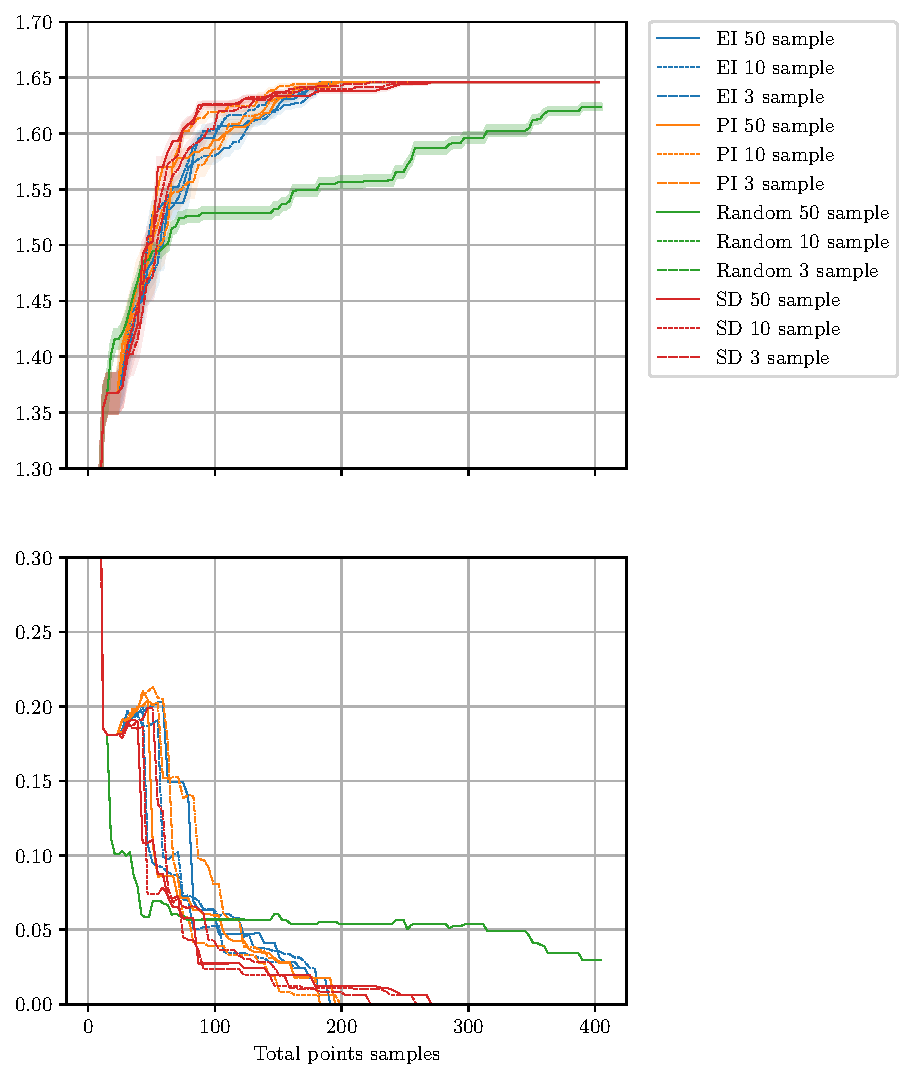
\includegraphics[width=\textwidth]{\dataset/search_algorithm_comparison_incremental_synthetic_3_output_incremental_long}
%		\caption{GPAR 3 training checkpoints model}
%	\end{subfigure}
%	\begin{subfigure}{0.48\textwidth}
%		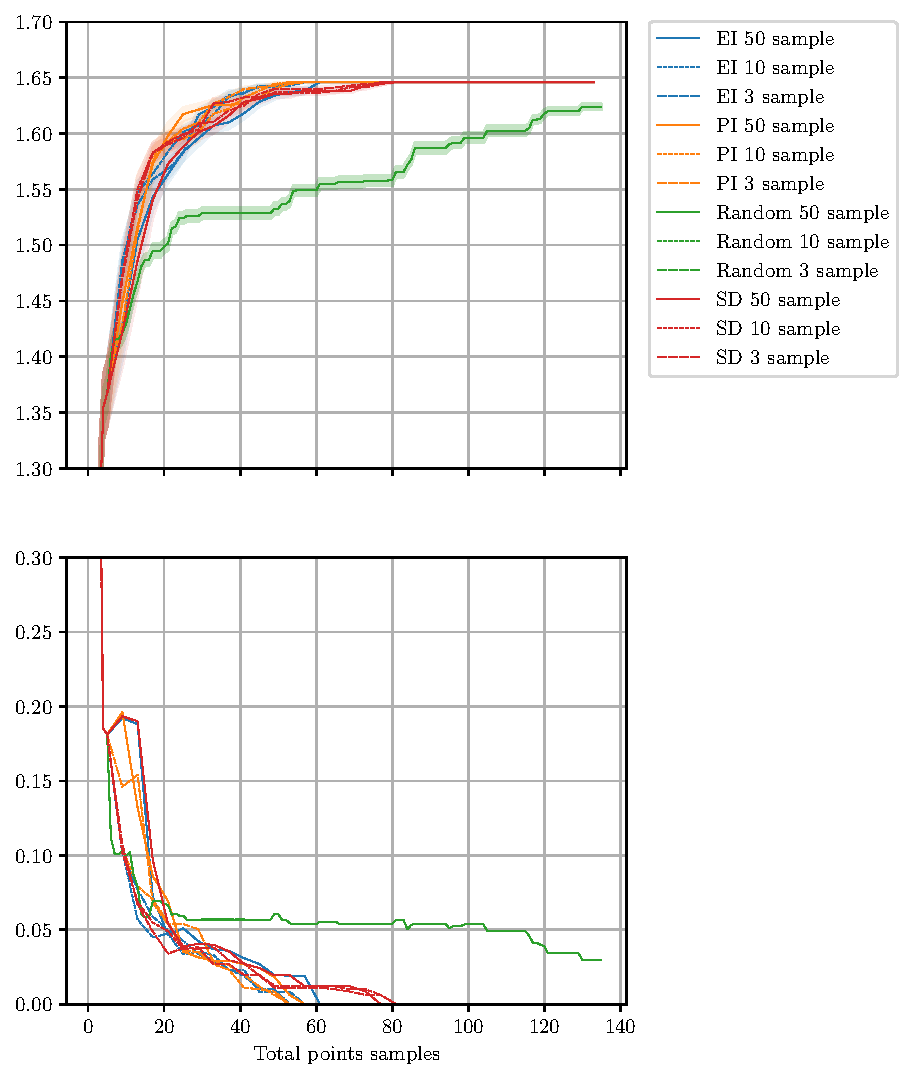
\includegraphics[width=\textwidth]{\dataset/search_algorithm_comparison_incremental_synthetic_3_output_long}
%		\caption{Final performance only model}
%	\end{subfigure}
%	\caption{The search efficiency of tested methods for MLP BNNs on the \dataname\quad dataset. Acquisition functions used are Expected Improvement (EI), Probability of Improvement (PI), Upper Confidence Bound (SD) and random search. 50, 10, and 3 samples were tried for estimating the mean and variance of the GP posterior function.}
%	\label{fig:searches_\dataset}
%\end{figure}

%\begin{figure}[p]
%	\def\dataset{\bostonvar}
%	\def\dataname{\bostonname}
%	\begin{subfigure}{0.48\textwidth}
%		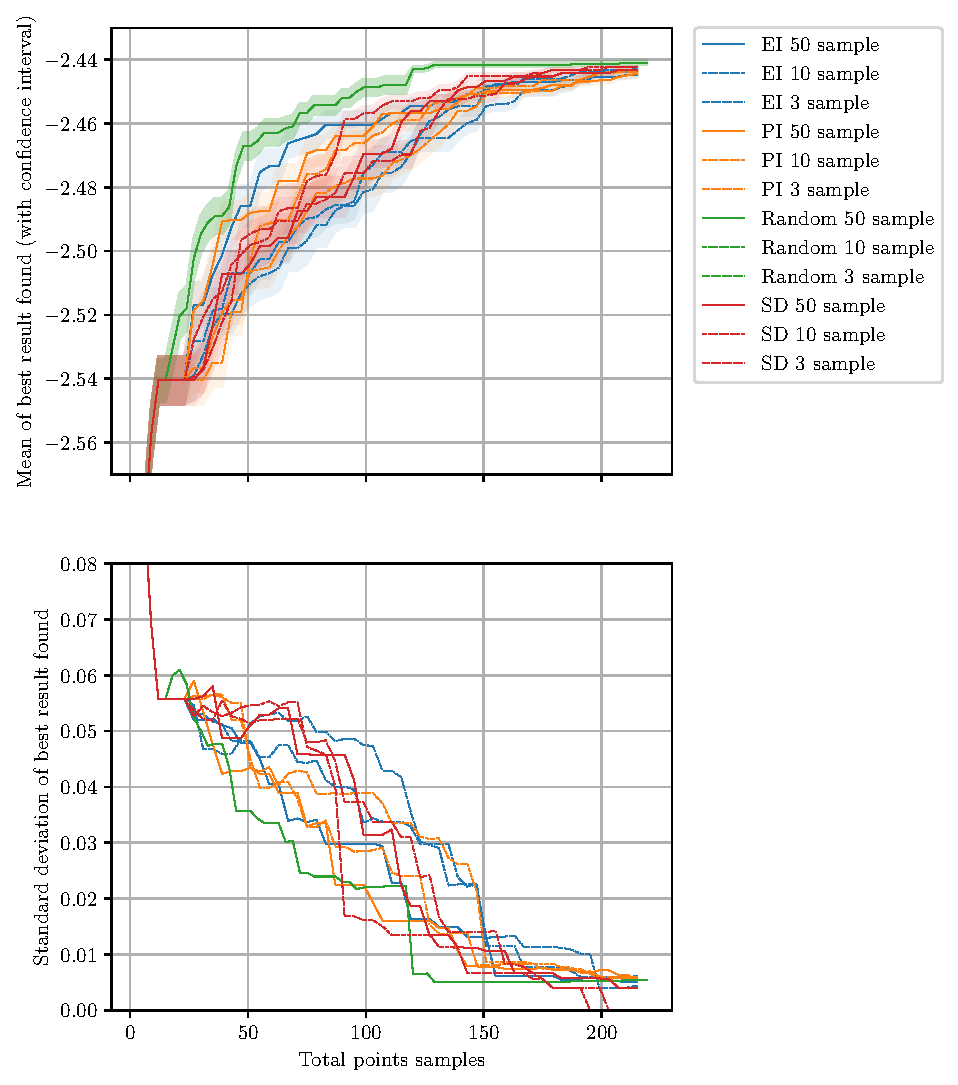
\includegraphics[width=\textwidth]{\dataset/search_algorithm_comparison_output_incremental_long}
%		\caption{\dataname}
%		\label{fig:hidden_width_\dataset}
%	\end{subfigure}
%	\def\dataset{\concretevar}
%	\def\dataname{\concretename}
%	\begin{subfigure}{0.48\textwidth}
%		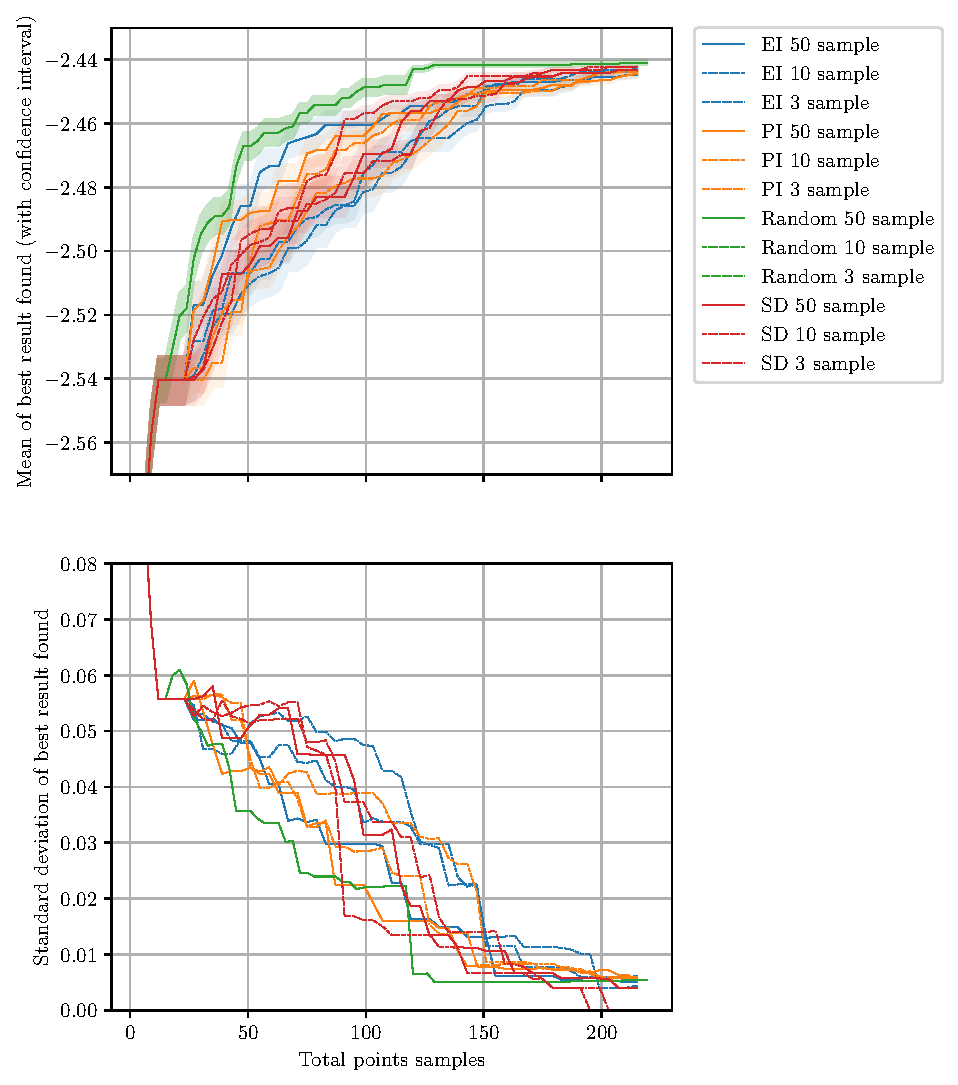
\includegraphics[width=\textwidth]{\dataset/search_algorithm_comparison_output_incremental_long}
%		\caption{\dataname}
%		\label{fig:hidden_width_\dataset}
%	\end{subfigure}
%	
%	\def\dataset{\energyvar}
%	\def\dataname{\energyname}
%	\begin{subfigure}{0.48\textwidth}
%		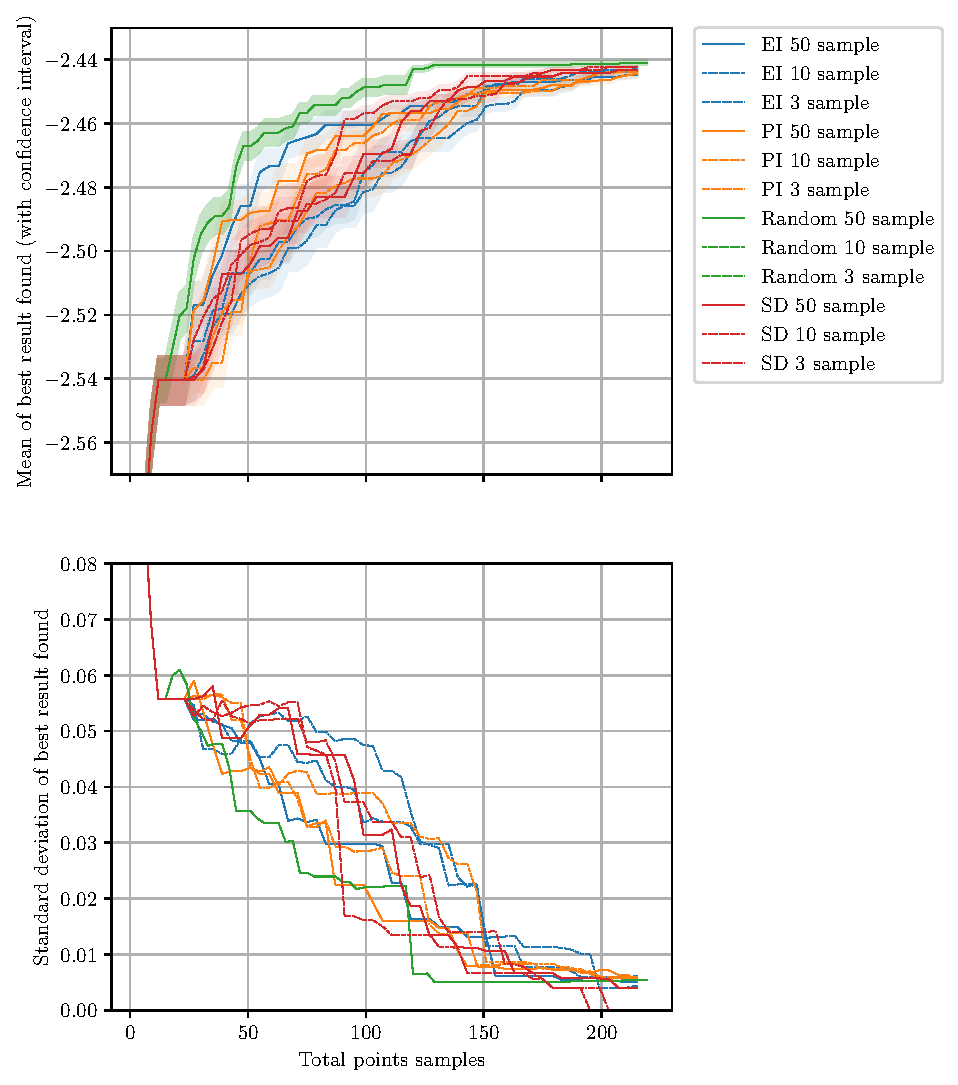
\includegraphics[width=\textwidth]{\dataset/search_algorithm_comparison_output_incremental_long}
%		\caption{\dataname}
%		\label{fig:hidden_width_\dataset}
%	\end{subfigure}
%	\def\dataset{\kinvar}
%	\def\dataname{\kinname}
%	\begin{subfigure}{0.48\textwidth}
%		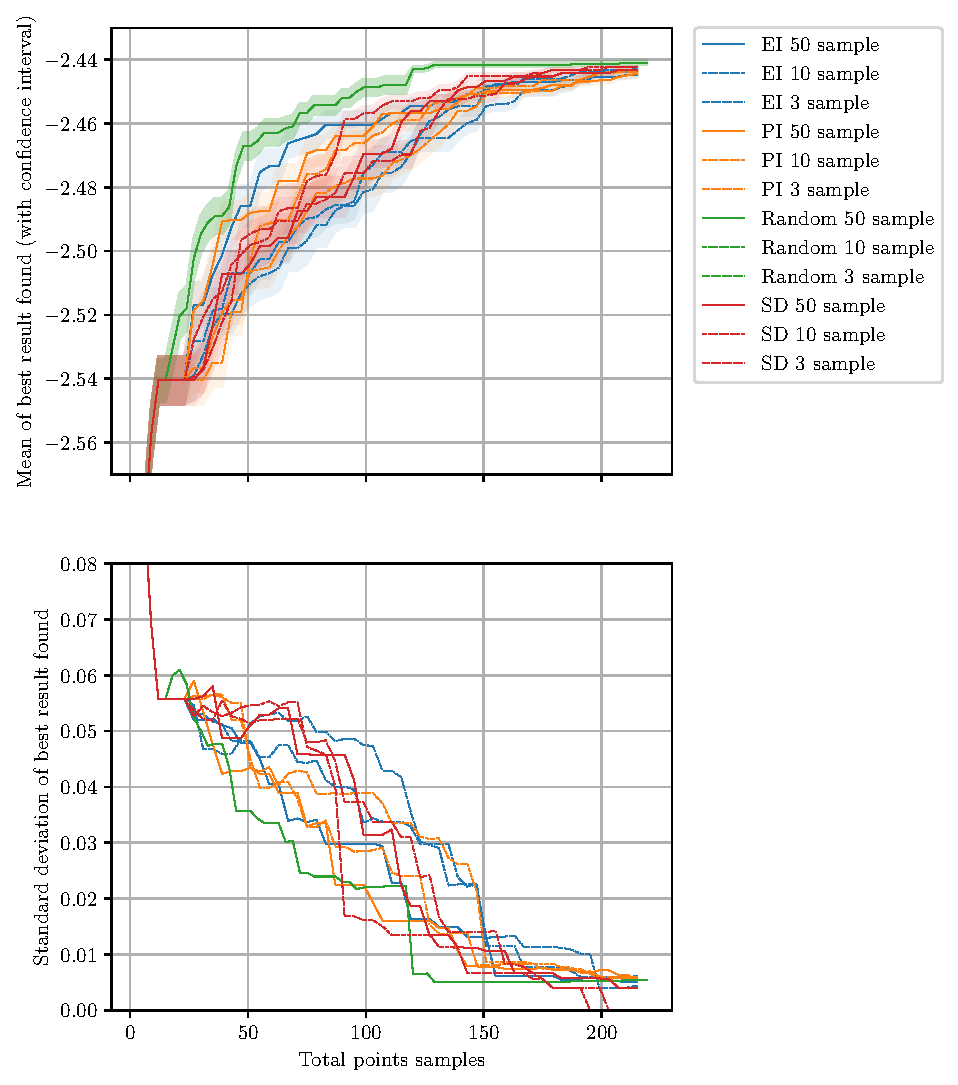
\includegraphics[width=\textwidth]{\dataset/search_algorithm_comparison_output_incremental_long}
%		\caption{\dataname}
%		\label{fig:hidden_width_\dataset}
%	\end{subfigure}
%	\caption{The search efficiency of searching the architecture space of MLP BNNs on various datasets, utilising the GPAR method with 3 checkpoints of training monitored. Acquisition function used are Expected Improvement (EI), Probability of Improvement (PI), Upper Confidence Bound (SD) and random search. 50, 10, and 3 samples were tried for estimating the mean and variance of the GP posterior function.}
%	\label{fig:gpar_1}
%\end{figure}
%
%\begin{figure}[p]
%	\def\dataset{\powervar}
%	\def\dataname{\powername}
%	\begin{subfigure}{0.48\textwidth}
%		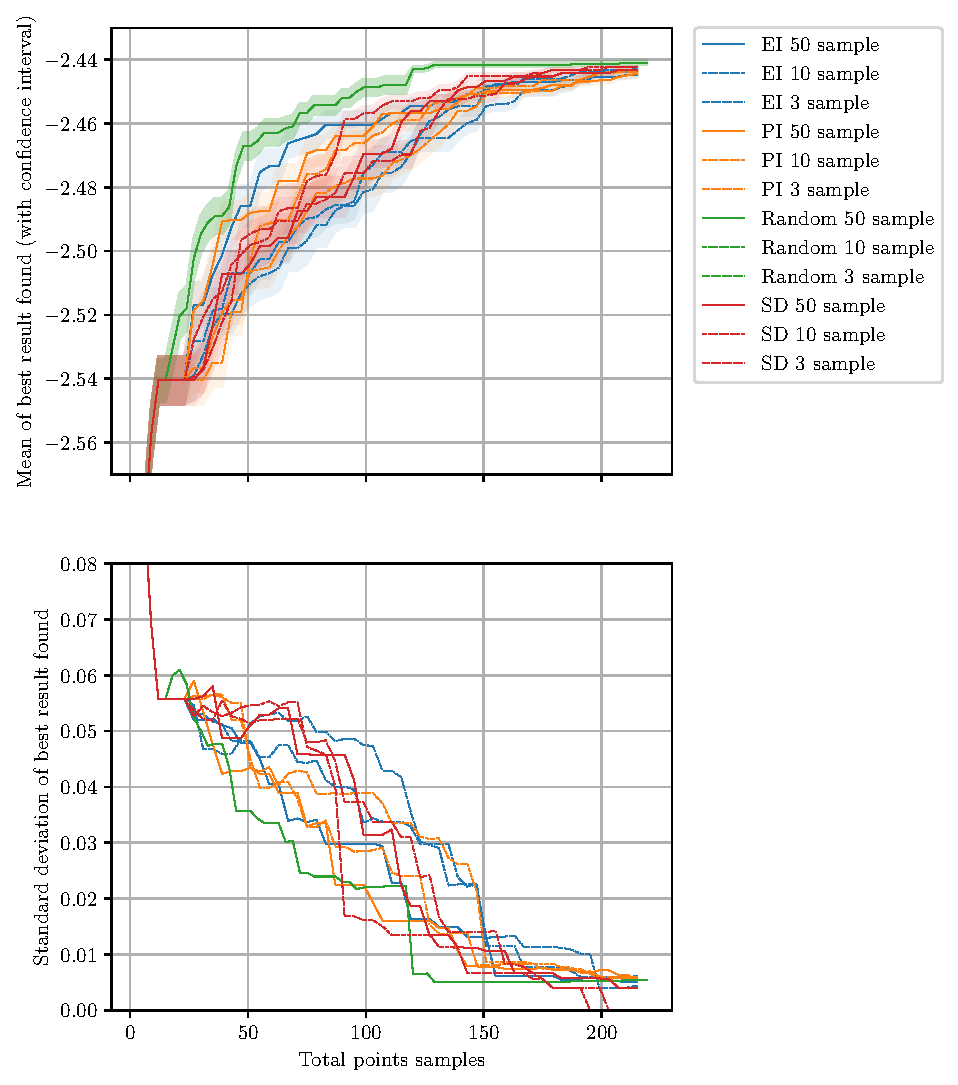
\includegraphics[width=\textwidth]{\dataset/search_algorithm_comparison_output_incremental_long}
%		\caption{\dataname}
%		\label{fig:hidden_width_\dataset}
%	\end{subfigure}
%%	\def\dataset{\proteinvar}
%%	\def\dataname{\proteinname}
%%	\begin{subfigure}{0.48\textwidth}
%%		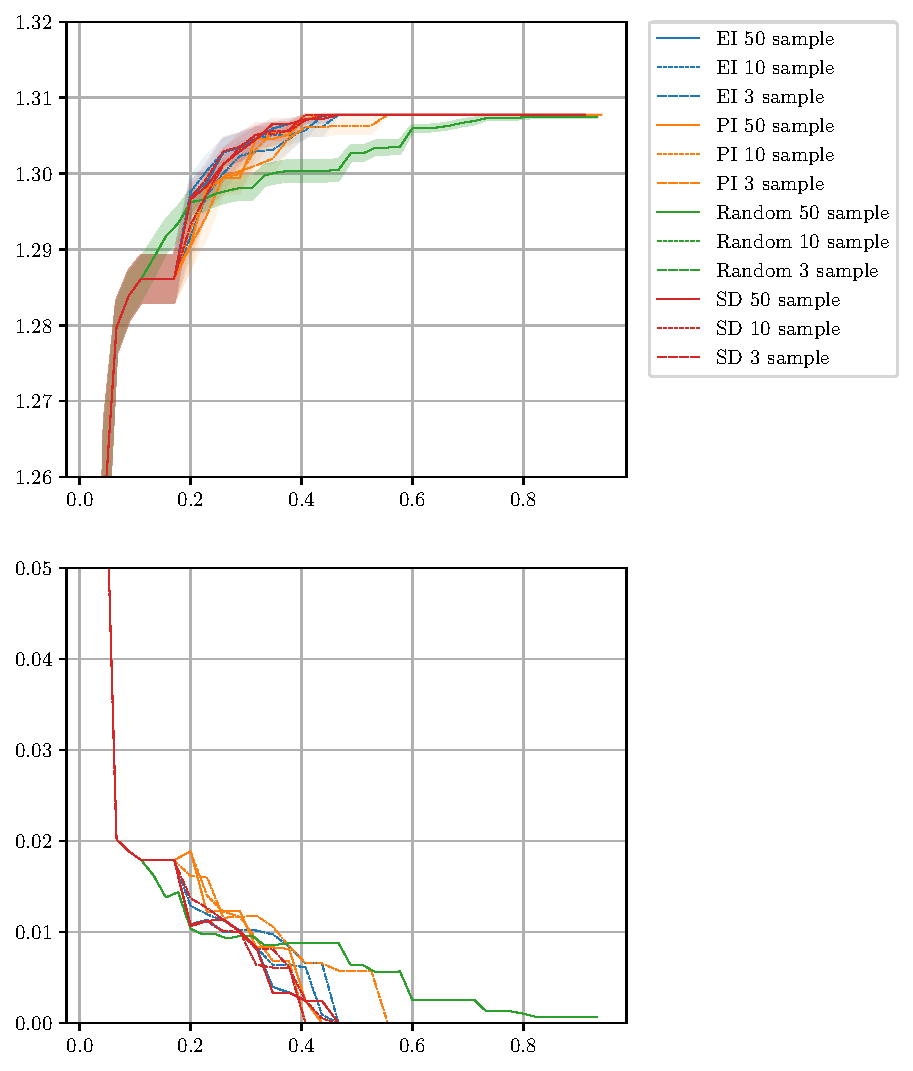
\includegraphics[width=\textwidth]{\dataset/search_algorithm_comparison}
%%		\caption{\dataname}
%%		\label{fig:pruning_\dataset}
%%	\end{subfigure}
%	
%	\def\dataset{\winevar}
%	\def\dataname{\winename}
%	\begin{subfigure}{0.48\textwidth}
%		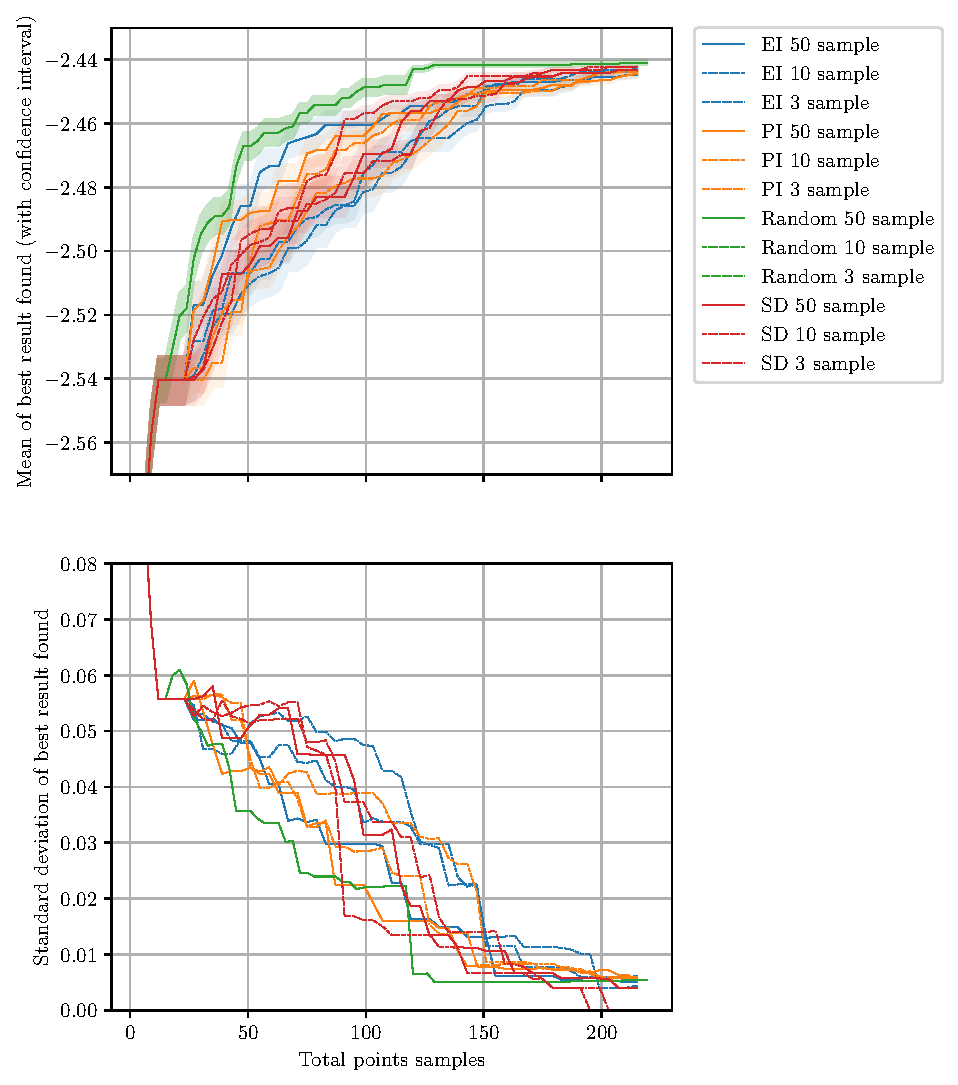
\includegraphics[width=\textwidth]{\dataset/search_algorithm_comparison_output_incremental_long}
%		\caption{\dataname}
%		\label{fig:hidden_width_\dataset}
%	\end{subfigure}
%	\def\dataset{\yachtnvar}
%	\def\dataname{\yachtname}
%	\begin{subfigure}{0.48\textwidth}
%		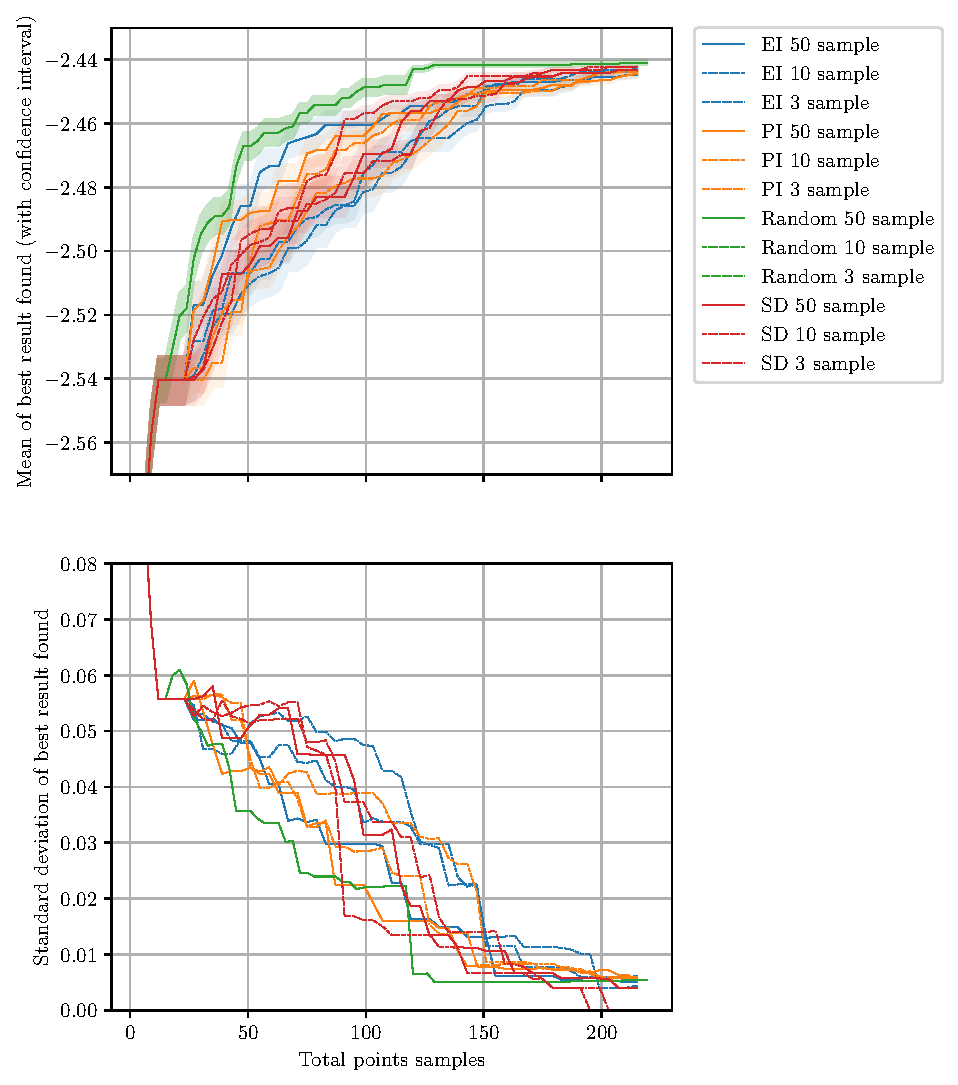
\includegraphics[width=\textwidth]{\dataset/search_algorithm_comparison_output_incremental_long}
%		\caption{\dataname}
%		\label{fig:hidden_width_\dataset}
%	\end{subfigure}
%	
%	\caption{The search efficiency of searching the architecture space of MLP BNNs on various datasets, utilising the GPAR method with 3 checkpoints of training monitored. Acquisition function used are Expected Improvement (EI), Probability of Improvement (PI), Upper Confidence Bound (SD) and random search. 50, 10, and 3 samples were tried for estimating the mean and variance of the GP posterior function.}
%	\label{fig:gpar_2}
%\end{figure}
%
%\begin{figure}[p]
%	\def\dataset{\bostonvar}
%	\def\dataname{\bostonname}
%	\begin{subfigure}{0.48\textwidth}
%		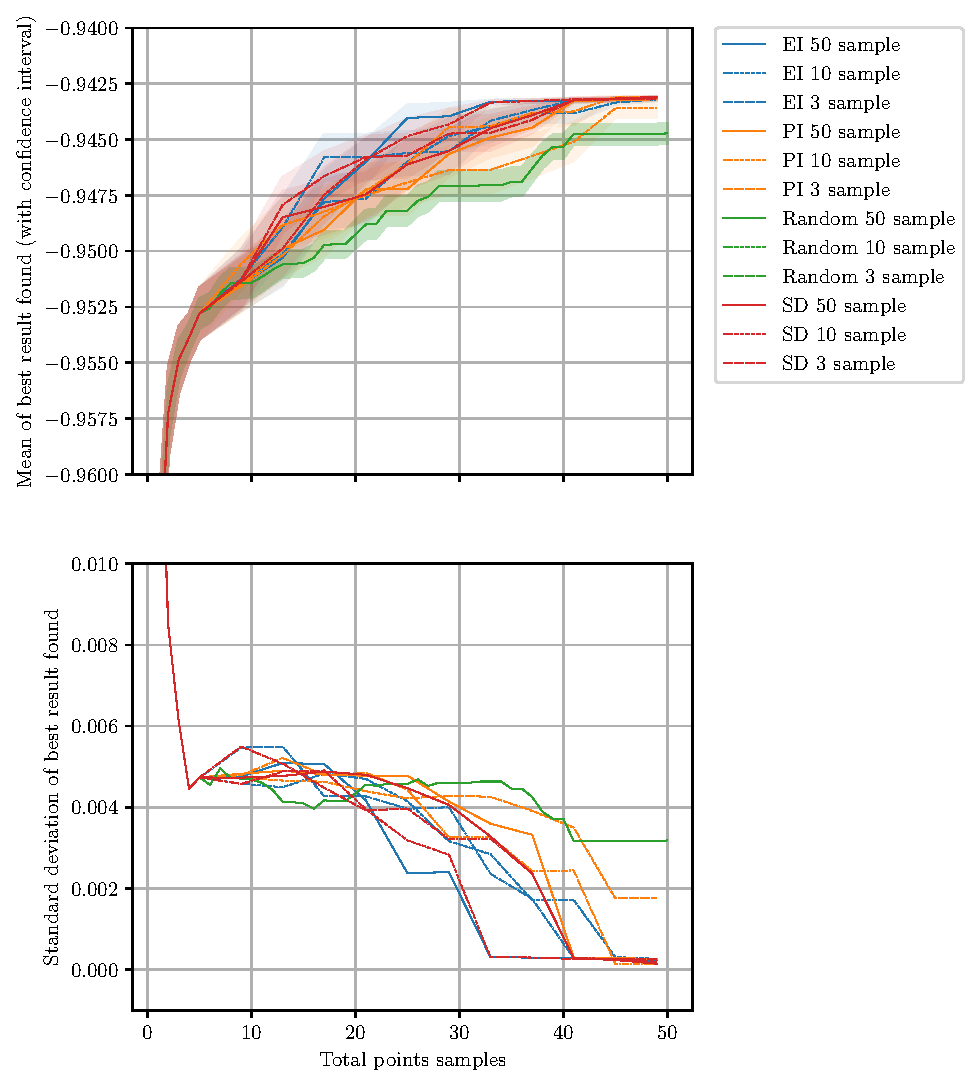
\includegraphics[width=\textwidth]{\dataset/search_algorithm_comparison_output_long}
%		\caption{\dataname}
%		\label{fig:hidden_width_\dataset}
%	\end{subfigure}
%	\def\dataset{\concretevar}
%	\def\dataname{\concretename}
%	\begin{subfigure}{0.48\textwidth}
%		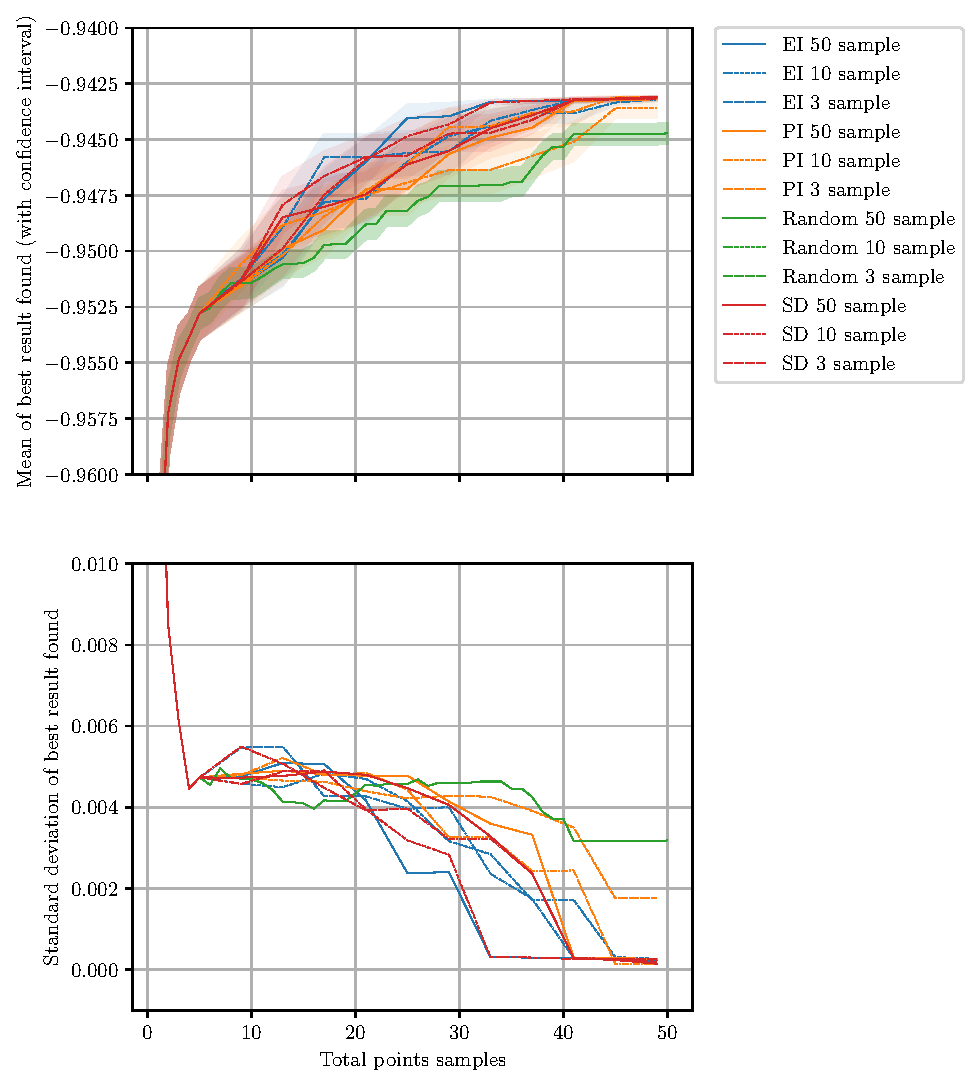
\includegraphics[width=\textwidth]{\dataset/search_algorithm_comparison_output_long}
%		\caption{\dataname}
%		\label{fig:hidden_width_\dataset}
%	\end{subfigure}
%	
%	\def\dataset{\energyvar}
%	\def\dataname{\energyname}
%	\begin{subfigure}{0.48\textwidth}
%		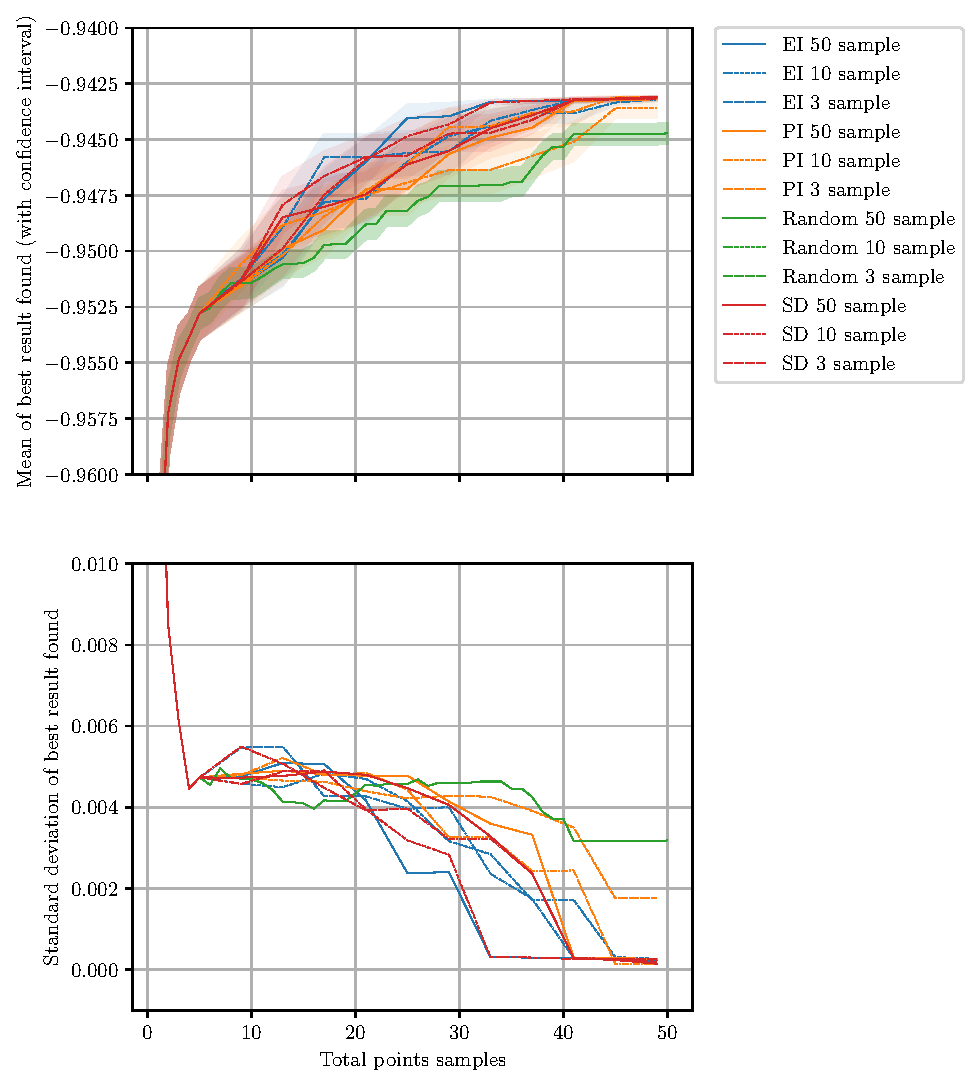
\includegraphics[width=\textwidth]{\dataset/search_algorithm_comparison_output_long}
%		\caption{\dataname}
%		\label{fig:hidden_width_\dataset}
%	\end{subfigure}
%	\def\dataset{\kinvar}
%	\def\dataname{\kinname}
%	\begin{subfigure}{0.48\textwidth}
%		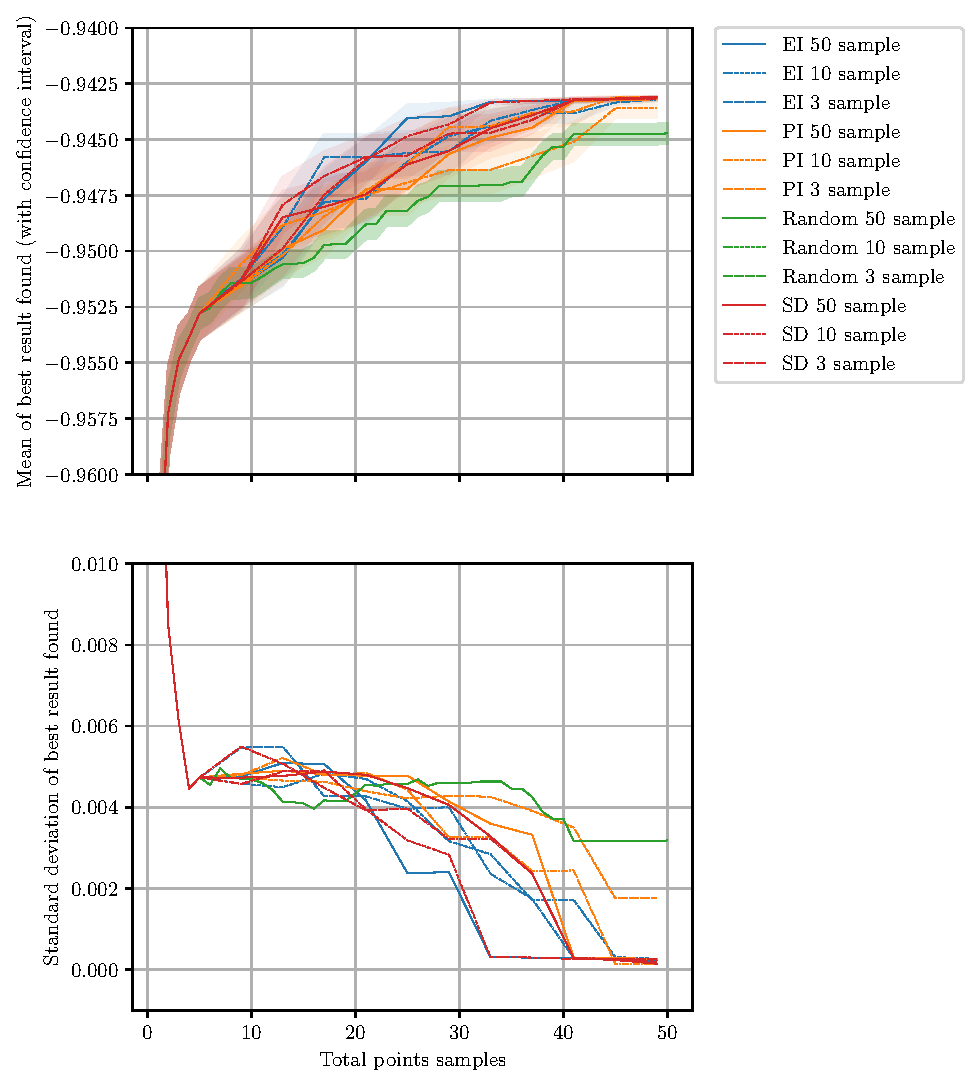
\includegraphics[width=\textwidth]{\dataset/search_algorithm_comparison_output_long}
%		\caption{\dataname}
%		\label{fig:hidden_width_\dataset}
%	\end{subfigure}
%	\caption{The search efficiency of searching the architecture space of MLP BNNs on various datasets, utilising the GPAR method with 3 checkpoints of training monitored. Acquisition function used are Expected Improvement (EI), Probability of Improvement (PI), Upper Confidence Bound (SD) and random search. 50, 10, and 3 samples were tried for estimating the mean and variance of the GP posterior function.}
%	\label{fig:final_1}
%\end{figure}
%
%\begin{figure}[p]
%	\def\dataset{\powervar}
%	\def\dataname{\powername}
%	\begin{subfigure}{0.48\textwidth}
%		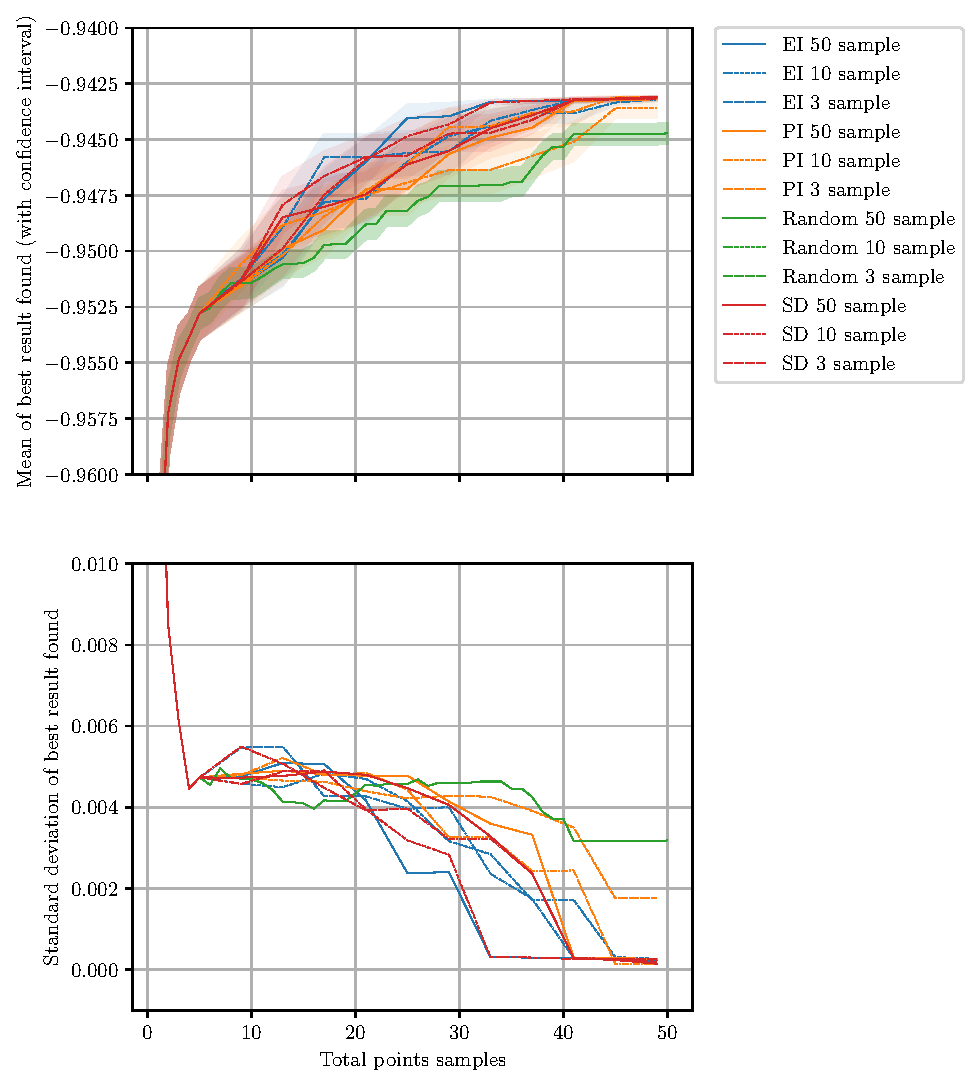
\includegraphics[width=\textwidth]{\dataset/search_algorithm_comparison_output_long}
%		\caption{\dataname}
%		\label{fig:hidden_width_\dataset}
%	\end{subfigure}
%	%	\def\dataset{\proteinvar}
%	%	\def\dataname{\proteinname}
%	%	\begin{subfigure}{0.48\textwidth}
%	%		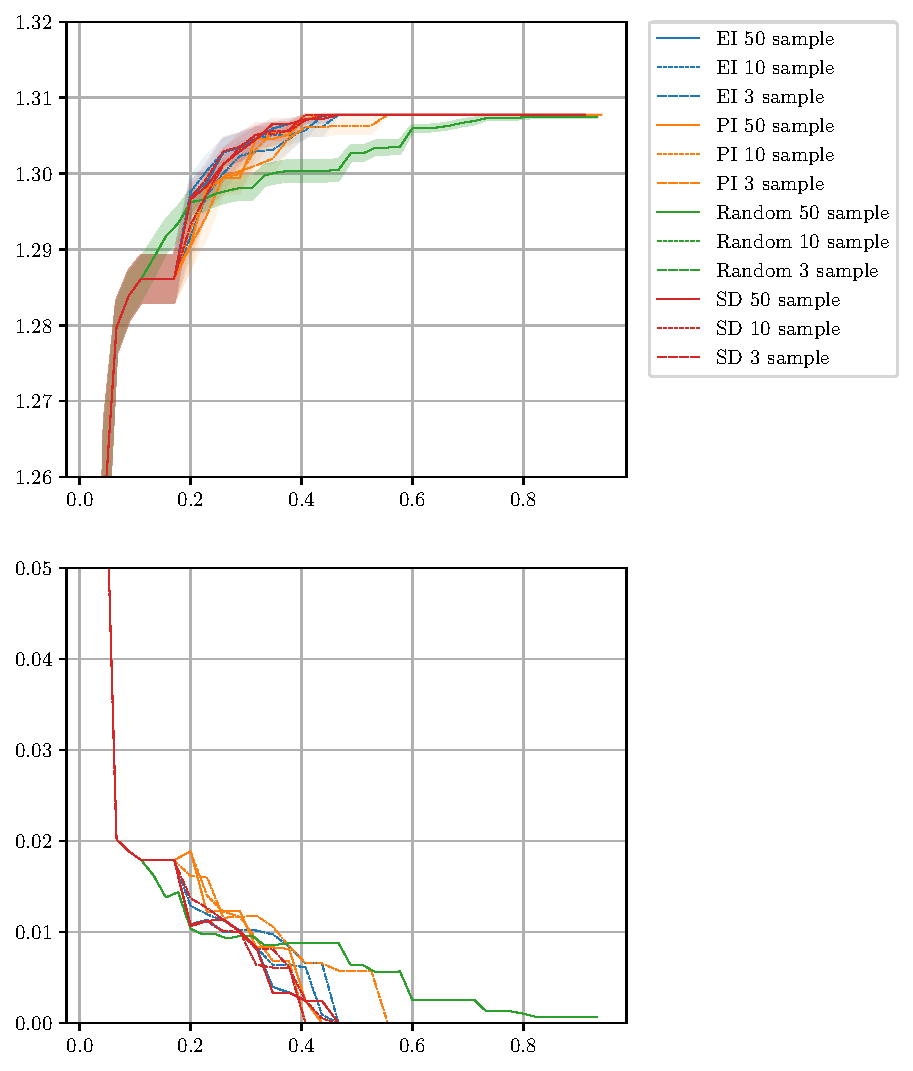
\includegraphics[width=\textwidth]{\dataset/search_algorithm_comparison}
%	%		\caption{\dataname}
%	%		\label{fig:pruning_\dataset}
%	%	\end{subfigure}
%	
%	\def\dataset{\winevar}
%	\def\dataname{\winename}
%	\begin{subfigure}{0.48\textwidth}
%		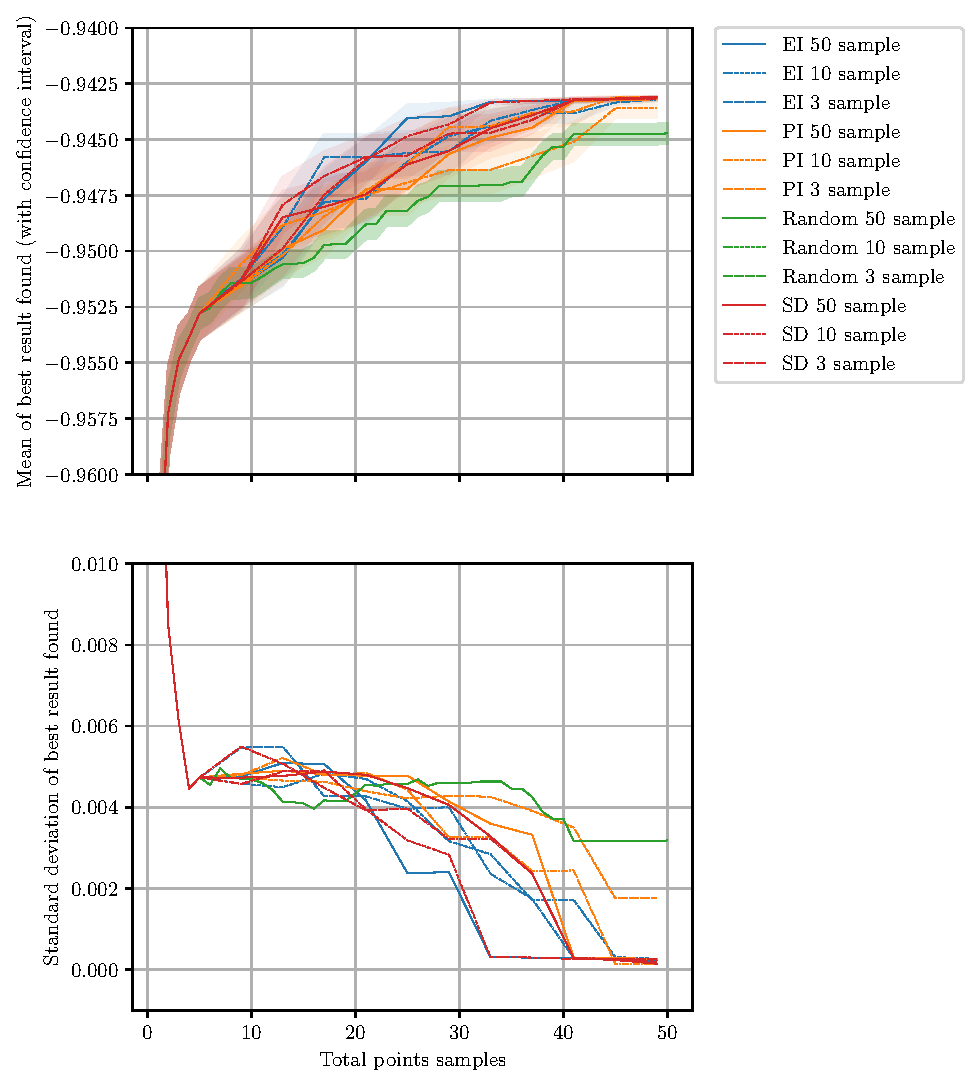
\includegraphics[width=\textwidth]{\dataset/search_algorithm_comparison_output_long}
%		\caption{\dataname}
%		\label{fig:hidden_width_\dataset}
%	\end{subfigure}
%	\def\dataset{\yachtnvar}
%	\def\dataname{\yachtname}
%	\begin{subfigure}{0.48\textwidth}
%		\includegraphics[width=\textwidth]{\dataset/search_algorithm_comparison_output_long}
%		\caption{\dataname}
%		\label{fig:hidden_width_\dataset}
%	\end{subfigure}
%	
%	\caption{The search efficiency of searching the architecture space of MLP BNNs on various datasets, utilising the GPAR method with 3 checkpoints of training monitored. Acquisition function used are Expected Improvement (EI), Probability of Improvement (PI), Upper Confidence Bound (SD) and random search. 50, 10, and 3 samples were tried for estimating the mean and variance of the GP posterior function.}
%	\label{fig:final_2}
%\end{figure}

\begin{figure}[p]
	\def\dataset{\bostonvar}
	\def\dataname{\bostonname}
	\begin{subfigure}{0.48\textwidth}
		\includegraphics[width=\textwidth]{\dataset/search_algorithm_comparison_output_incremental_long}
		\caption{GPAR 3 training checkpoints model}
	\end{subfigure}
	\begin{subfigure}{0.48\textwidth}
		\includegraphics[width=\textwidth]{\dataset/search_algorithm_comparison_output_long}
		\caption{Final performance only model}
	\end{subfigure}
	\caption{The search efficiency of tested methods for MLP BNNs on the \dataname\quad dataset. Acquisition functions used are Expected Improvement (EI), Probability of Improvement (PI), Upper Confidence Bound (SD) and random search. 50, 10, and 3 samples were tried for estimating the mean and variance of the GP posterior function.}
	\label{fig:searches_\dataset}
\end{figure}

\begin{figure}[p]
	\def\dataset{\concretevar}
	\def\dataname{\concretename}
	\begin{subfigure}{0.48\textwidth}
		\includegraphics[width=\textwidth]{\dataset/search_algorithm_comparison_output_incremental_long}
		\caption{GPAR 3 training checkpoints model}
	\end{subfigure}
	\begin{subfigure}{0.48\textwidth}
		\includegraphics[width=\textwidth]{\dataset/search_algorithm_comparison_output_long}
		\caption{Final performance only model}
	\end{subfigure}
	\caption{The search efficiency of tested methods for MLP BNNs on the \dataname\quad dataset. Acquisition functions used are Expected Improvement (EI), Probability of Improvement (PI), Upper Confidence Bound (SD) and random search. 50, 10, and 3 samples were tried for estimating the mean and variance of the GP posterior function.}
	\label{fig:searches_\dataset}
\end{figure}

\begin{figure}[p]
	\def\dataset{\energyvar}
	\def\dataname{\energyname}
	\begin{subfigure}{0.48\textwidth}
		\includegraphics[width=\textwidth]{\dataset/search_algorithm_comparison_output_incremental_long}
		\caption{GPAR 3 training checkpoints model}
	\end{subfigure}
	\begin{subfigure}{0.48\textwidth}
		\includegraphics[width=\textwidth]{\dataset/search_algorithm_comparison_output_long}
		\caption{Final performance only model}
	\end{subfigure}
	\caption{The search efficiency of tested methods for MLP BNNs on the \dataname\quad dataset. Acquisition functions used are Expected Improvement (EI), Probability of Improvement (PI), Upper Confidence Bound (SD) and random search. 50, 10, and 3 samples were tried for estimating the mean and variance of the GP posterior function.}
	\label{fig:searches_\dataset}
\end{figure}

\begin{figure}[p]
	\def\dataset{\kinvar}
	\def\dataname{\kinname}
	\begin{subfigure}{0.48\textwidth}
		\includegraphics[width=\textwidth]{\dataset/search_algorithm_comparison_output_incremental_long}
		\caption{GPAR 3 training checkpoints model}
	\end{subfigure}
	\begin{subfigure}{0.48\textwidth}
		\includegraphics[width=\textwidth]{\dataset/search_algorithm_comparison_output_long}
		\caption{Final performance only model}
	\end{subfigure}
	\caption{The search efficiency of tested methods for MLP BNNs on the \dataname\quad dataset. Acquisition functions used are Expected Improvement (EI), Probability of Improvement (PI), Upper Confidence Bound (SD) and random search. 50, 10, and 3 samples were tried for estimating the mean and variance of the GP posterior function.}
	\label{fig:searches_\dataset}
\end{figure}

\begin{figure}[p]
	\def\dataset{\powervar}
	\def\dataname{\powername}
	\begin{subfigure}{0.48\textwidth}
		\includegraphics[width=\textwidth]{\dataset/search_algorithm_comparison_output_incremental_long}
		\caption{GPAR 3 training checkpoints model}
	\end{subfigure}
	\begin{subfigure}{0.48\textwidth}
		\includegraphics[width=\textwidth]{\dataset/search_algorithm_comparison_output_long}
		\caption{Final performance only model}
	\end{subfigure}
	\caption{The search efficiency of tested methods for MLP BNNs on the \dataname\quad dataset. Acquisition functions used are Expected Improvement (EI), Probability of Improvement (PI), Upper Confidence Bound (SD) and random search. 50, 10, and 3 samples were tried for estimating the mean and variance of the GP posterior function.}
	\label{fig:searches_\dataset}
\end{figure}

\begin{figure}[p]
	\def\dataset{\proteinvar}
	\def\dataname{\proteinname}
	\begin{subfigure}{0.48\textwidth}
		\includegraphics[width=\textwidth]{\dataset/search_algorithm_comparison_output_incremental_long}
		\caption{GPAR 3 training checkpoints model}
	\end{subfigure}
	\begin{subfigure}{0.48\textwidth}
		\includegraphics[width=\textwidth]{\dataset/search_algorithm_comparison_output_long}
		\caption{Final performance only model}
	\end{subfigure}
	\caption{The search efficiency of tested methods for MLP BNNs on the \dataname\quad dataset. Acquisition functions used are Expected Improvement (EI), Probability of Improvement (PI), Upper Confidence Bound (SD) and random search. 50, 10, and 3 samples were tried for estimating the mean and variance of the GP posterior function.}
	\label{fig:searches_\dataset}
\end{figure}

\begin{figure}[p]
	\def\dataset{\winevar}
	\def\dataname{\winename}
	\begin{subfigure}{0.48\textwidth}
		\includegraphics[width=\textwidth]{\dataset/search_algorithm_comparison_output_incremental_long}
		\caption{GPAR 3 training checkpoints model}
	\end{subfigure}
	\begin{subfigure}{0.48\textwidth}
		\includegraphics[width=\textwidth]{\dataset/search_algorithm_comparison_output_long}
		\caption{Final performance only model}
	\end{subfigure}
	\caption{The search efficiency of tested methods for MLP BNNs on the \dataname\quad dataset. Acquisition functions used are Expected Improvement (EI), Probability of Improvement (PI), Upper Confidence Bound (SD) and random search. 50, 10, and 3 samples were tried for estimating the mean and variance of the GP posterior function.}
	\label{fig:searches_\dataset}
\end{figure}

\begin{figure}[p]
	\def\dataset{\yachtnvar}
	\def\dataname{\yachtname}
	\begin{subfigure}{0.48\textwidth}
		\includegraphics[width=\textwidth]{\dataset/search_algorithm_comparison_output_incremental_long}
		\caption{GPAR 3 training checkpoints model}
	\end{subfigure}
	\begin{subfigure}{0.48\textwidth}
		\includegraphics[width=\textwidth]{\dataset/search_algorithm_comparison_output_long}
		\caption{Final performance only model}
	\end{subfigure}
	\caption{The search efficiency of tested methods for MLP BNNs on the \dataname\quad dataset. Acquisition functions used are Expected Improvement (EI), Probability of Improvement (PI), Upper Confidence Bound (SD) and random search. 50, 10, and 3 samples were tried for estimating the mean and variance of the GP posterior function.}
	\label{fig:searches_\dataset}
\end{figure}
